% ============================================================================
% Supplementary Material
% A Critical Assessment of AM-Specific Damage Descriptors for Fracture
% Prediction: Strict Cross-Validation and Applicability Limits
% Detailed nonlocal-regularization study moved from the main text (Section
% "Nonlocal damage regularization of the full-field reference").
% ============================================================================

\documentclass[12pt,a4paper,twocolumn]{article}
\usepackage[utf8]{inputenc}
\usepackage[T1]{fontenc}
\usepackage{amsmath,amssymb,amsfonts}
\usepackage{graphicx}
\usepackage{booktabs}
\usepackage{hyperref}
\usepackage{float}
\usepackage{array}
\usepackage{multirow}
\usepackage{xcolor}
\usepackage{siunitx}
\usepackage{tikz}
\usetikzlibrary{arrows.meta,positioning}
\setlength{\oddsidemargin}{-0.39mm}
\setlength{\evensidemargin}{-0.39mm}
\setlength{\textwidth}{160mm}
\setlength{\topmargin}{-10.6mm}
\setlength{\textheight}{247mm}
\hypersetup{colorlinks=true,linkcolor=blue,citecolor=blue,urlcolor=blue}

\providecommand{\ang}[1]{\ensuremath{#1^{\circ}}}

\title{\textbf{Supplementary Material: Detailed Nonlocal Regularization, Extended Cross-Validation, Code Verification, Reproducibility Bindings and Public-Data Assessment}}
\author{[First Author] \thinspace [Second Author]}
\date{}

\begin{document}
\maketitle

\section*{S1. Nonlocal damage regularization of the full-field reference}

The main text (Section~``Nonlocal damage regularization of the full-field reference'') reports only the
headline conclusion of this study; the full route selection, implementation verification, tables and
diagnostics are collected here. The full-field-reference section of the main paper quantifies the surrogate's
bias against full-field references, but it leaves two things open: the in-house full-field reference is
itself a local-damage model, so its own mesh dependence is unmeasured, and the strain localization at which
the coupled FFT iteration diverges is a boundary of the reference rather than of the surrogate. This study
addresses both by adding a strain-localization regularization to the in-house three-dimensional CPFEM
reference and measuring what it does and what it does not do. All runs use the locked material and protocol
of the reference (Ti-6Al-4V at $\ang{0}$ unless stated, $S_0 = 0.32$\,MPa, $D_c = 0.42$, damage threshold
$p_D = 0.05$, $n_{\mathrm{sub}} = 30$, strain rate $10^{-3}\,\mathrm{s}^{-1}$, seed 42,
$\Delta\varepsilon = 10^{-3}$), and the fracture criterion is unchanged: $D_{\mathrm{agg}} \ge D_c$ or
localization onset, exactly as in the main-text full-field section. Fifteen runs constitute the study.

\paragraph{Route selection.} Three regularization routes were evaluated against the constraints of this
solver---hexahedral elements, a damped Newton iteration with a finite-difference numerical tangent,
$n_{\mathrm{sub}} = 30$ constitutive sub-steps re-evaluated inside every residual, and no scalar-field degree
of freedom or sparse linear solver. An \emph{integral-type nonlocal} formulation was selected. The local
equivalent plastic strain that gates and drives damage is replaced by its weighted neighbourhood average, $W$
being a row-normalized Gaussian kernel of internal length $\ell_c$ truncated at $3\ell_c$ and computed once
from the integration-point geometry; because the operator is a state-independent constant matrix, it adds no
Newton unknowns, does not change the residual dimension, and enters the numerical tangent automatically, since
the tangent differentiates the same residual that now contains the kernel. The measured overhead is a factor
of $1.029$ on the tangent and $1.039$ on the residual at 27 grains, and $1.060$/$1.038$ at 64 grains, the two
ratios agreeing to within about two percentage points, which is what one expects if the coupling is genuinely
carried through the tangent rather than merely added to the residual. An \emph{implicit gradient} (Helmholtz)
filter was rejected because it would make the driving variable implicit and would need a scalar-field assembly
and a sparse solver the framework does not have (about $+64\%$ on the tangent budget). An \emph{Allen--Cahn
phase-field} route was not implemented: it needs additional Newton unknowns, a gradient-energy term,
interface-parameter calibration and, decisively, a redefinition of the fracture criterion, which would break
consistency with the locked full-field results. It is declared a higher-fidelity follow-on and is not
substituted for by any proxy anywhere in this work.

\paragraph{Verification of the implementation.} The nonlocal solver was verified rather than asserted. With
$W$ set to the identity the nonlocal code is \emph{bit-identical} to the local solver---same strain, stress
and damage at every step, zero difference in the fracture strain---on both a damage-free path and a branch
with damage active; and at $\Delta\varepsilon = 2\times10^{-3}$ it reproduces the archived R13 run step by
step, with identical damage history and identical Newton iteration counts at every print point. The single
difference from the archived value is a truncation convention rather than a disagreement: R13 recorded the
last converged increment ($\varepsilon_f = 0.1389$, $D_{\mathrm{agg}} = 0.4157$), whereas these runs continue
to an actual $D_{\mathrm{agg}} \ge D_c$ crossing and give $\varepsilon_f^{\mathrm{local}} = 0.13967$, a
$+0.55\%$ shift. The local full-field fracture strain is also step-converged: $10^{-3}$ and $2\times10^{-3}$
give $0.139666$ and $0.139666$, identical to twelve digits. The $\ell_c \to 0$ limit of the kernel is
recovered as well: at $\ell_c = 0.0625$ the kernel is essentially the identity ($n_{\mathrm{eff}} = 1.03$,
self-weight $0.988$) and $\varepsilon_f = 0.13971$, i.e.\ $+0.031\%$ from the local value. Together the
identity limit, the archived-run reproduction and the $\ell_c \to 0$ limit are three independent checks that
the operator and its coupling are implemented correctly.

\begin{table}[htbp]
\centering
\caption{Internal-length scan of the nonlocal regularization at the production protocol (Ti-6Al-4V, $\ang{0}$,
27 grains, $\Delta\varepsilon = 10^{-3}$). $n_{\mathrm{eff}} = 1/\sum_j W_{ij}^2$ is the effective number of
integration points averaged, given both in integration points and in grains (216 integration points $= 27$
grains), $W_{ii}$ is the self-weight of an integration point, and the last column is the measured damage
accumulation rate over $\varepsilon \in [0.05, 0.10]$. All runs terminate on the $D_{\mathrm{agg}} \ge D_c$
branch.}
\label{tab:nonlocal_lc}
\footnotesize
\setlength{\tabcolsep}{3pt}
\begin{tabular}{cccccc}
\toprule
$\ell_c/h$ & $n_{\mathrm{eff}}$ & $n_{\mathrm{eff}}/n_{\mathrm{g}}$ & $W_{ii}$ & $\varepsilon_f$ & $\dot{D}_{\mathrm{agg}}$ \\
\midrule
0 (local) & 1.00 & 0.13 & 1.000 & 0.13967 & 4.02 \\
0.1875 & 1.03 & 0.13 & 0.988 & 0.13971 & 4.02 \\
0.3750 & 3.76 & 0.47 & 0.492 & 0.14248 & 3.92 \\
0.7500 & 28.88 & 3.61 & 0.093 & 0.14924 & 3.39 \\
1.0000 & 55.45 & 6.93 & 0.047 & 0.15268 & 3.09 \\
\bottomrule
\multicolumn{6}{p{0.97\columnwidth}}{\footnotesize The $\ell_c \to 0$ limit returns the local value to within
$+0.031\%$ (row 2), and the fracture strain then rises monotonically with $\ell_c$, by $+2.02\%$ at
$\ell_c = 0.375h$ and $+9.32\%$ at one grain. The kernel diagnostics also bound how far this scan is
physically meaningful: at $\ell_c$ equal to one grain the average already covers $6.9$ grains of a 27-grain
RVE and an integration point retains only $4.7\%$ of its own value, so the regularization there has
degenerated towards homogenization.}
\end{tabular}
\end{table}

\paragraph{Mesh dependence: compressed by a factor of four to nine, not removed.} Table~\ref{tab:nonlocal_mesh}
states the first measurement of the full-field reference's own mesh dependence. Refining from 27 to 64 grains
under the identical protocol moves the \emph{local} fracture strain by $-15.92\%$ ($0.13967 \to 0.11744$), and
the failure branch changes with it: the 27-grain run ends on a smooth $D_{\mathrm{agg}} \ge D_c$ crossing while
the 64-grain run slips onto localization onset with the step size at its floor, $D_{\max} = 0.99$ (an
integration point at the damage cap) and $D_{\max}/D_{\mathrm{mean}} = 3.17$. Mesh refinement thus pushes the
local model back into an instability-dominated failure mode. With the nonlocal operator the same refinement
moves the fracture strain by $-1.75\%$ to $-3.97\%$ depending on how $\ell_c$ is carried across the meshes, all
nonlocal runs terminate on the same $D_{\mathrm{agg}} \ge D_c$ branch on both meshes, and the 64-grain runs
need only one to two step reductions. The regularization therefore compresses the mesh dependence by a factor
of four to nine and stabilizes the failure branch, but it does not eliminate the dependence: a residual
$2$--$4\%$ shift remains. Two points of honesty belong here. First, the residual shift is similar whether
$\ell_c$ is held fixed as a physical length or rescaled with the mesh, which indicates that it comes mainly
from the change of the RVE realization (a new random orientation set at 64 grains, with no periodicity) rather
than from the coupling of $\ell_c$ to the element size. Second, the mesh objectivity of the damage \emph{field}
is at least as informative as that of the scalar $\varepsilon_f$: at the common strain $\varepsilon = 0.10$ the
kernel-smoothed roughness and the peak-to-mean ratio are mesh-objective on the nonlocal field ($-2.4\%$ and
$-3.0\%$ between the two meshes) and clearly non-objective on the local field ($+19.9\%$ and $+43.9\%$), while
the mean first-order gradient still moves by $-29.4\%$ on the nonlocal field---that measure is defined on a
neighbourhood radius that itself changes with the mesh, so most of its mesh behaviour is an artefact of its own
definition and we do not use it as evidence either way.

\begin{table}[htbp]
\centering
\caption{Mesh dependence of the fracture strain of the three-dimensional full-field reference (Ti-6Al-4V,
$\ang{0}$), 27 versus 64 grains. ``Termination'' gives the fracture branch, $D_{\mathrm{agg}} \ge D_c$ or
localization onset. The nonlocal rows differ only in how $\ell_c$ is carried across the two meshes.}
\label{tab:nonlocal_mesh}
\footnotesize
\setlength{\tabcolsep}{3pt}
\begin{tabular}{p{0.20\columnwidth}p{0.09\columnwidth}p{0.09\columnwidth}ccr}
\toprule
$\ell_c$ carried as & $\ell_c/h$ (27) & $\ell_c/h$ (64) & $\varepsilon_f$ (27) & $\varepsilon_f$ (64) & $\Delta$ [\%] \\
\midrule
local, no kernel & -- & -- & 0.13967 & 0.11744 & $-15.92$ \\
fixed physical length & 1.00 & 1.33 & 0.15268 & 0.14932 & $-2.21$ \\
rescaled to one grain & 1.00 & 1.00 & 0.15268 & 0.14663 & $-3.97$ \\
fixed physical length ($\ell_c = 0.25$) & 0.75 & 1.00 & 0.14924 & 0.14663 & $-1.75$ \\
\bottomrule
\multicolumn{6}{p{0.97\columnwidth}}{\footnotesize 27 grains $= 3^3$, 64 grains $= 4^3$; the two meshes use
independent random orientation sets. The local pair also changes termination branch ($D_c$ crossing $\to$
localization onset); all three nonlocal pairs keep the $D_c$ crossing on both meshes.}
\end{tabular}
\end{table}

\paragraph{Effect on the Taylor bias band, and a structure that does not survive it.} Table~\ref{tab:nonlocal_bias}
places the regularized reference beside the locked bias band of the main text. Two statements are supported by
the measurement and one is not. The direction ordering survives: $\ang{0} > \ang{45} > \ang{90}$ holds in every
setting tested. And the band changes \emph{shape}, not merely width. In the local model the $\ang{45}$ and
$\ang{90}$ biases are negative while the $\ang{0}$ bias is positive, so the Taylor reference brackets the
full-field value from both sides---the structure the constraint-dependence argument of the main text rests on.
Strong nonlocalization raises the softer directions more than the $\ang{0}$ direction, and all three
orientations then overestimate Taylor: the band's lower edge moves from $-14.19\%$ to $+6.53\%$ and the
$\ang{45}$ entry from $-5.02\%$ to $+19.22\%$, while the width narrows only modestly, from 39.2 to 30.1
percentage points. The bracketing structure is therefore a property of the local reference at the present
internal length, not a robust feature of the surrogate, and we record it as a qualification of the band rather
than as support for it.

\begin{table*}[htbp]
\centering
\caption{Taylor bias of the three-dimensional full-field reference in three build orientations, with and
without the nonlocal regularization (Ti-6Al-4V, 27 grains, $\Delta\varepsilon = 10^{-3}$). The Taylor aggregate
is listed at both the strain increment of the locked reference ($2\times10^{-3}$) and the verified step
($10^{-3}$); the parenthesized biases of the full-field rows are against the \emph{locked} $2\times10^{-3}$
Taylor values.}
\label{tab:nonlocal_bias}
\footnotesize
\setlength{\tabcolsep}{3pt}
\begin{tabular}{p{0.34\textwidth}ccc}
\toprule
 & $\ang{0}$ & $\ang{45}$ & $\ang{90}$ \\
\midrule
Taylor aggregate, locked ($2\times10^{-3}$) & 0.11175 & 0.09226 & 0.07750 \\
Taylor aggregate, verified step ($10^{-3}$) & 0.07255 & 0.05421 & 0.04434 \\
Full-field local & 0.13967 ($+24.98$) & 0.08763 ($-5.02$) & 0.06650 ($-14.19$) \\
Full-field nonlocal, $\ell_c = 0.125$ & 0.14248 ($+27.50$) & 0.09178 ($-0.52$) & 0.06869 ($-11.37$) \\
Full-field nonlocal, $\ell_c = $ 1 grain & 0.15268 ($+36.63$) & 0.10999 ($+19.22$) & 0.08256 ($+6.53$) \\
\bottomrule
\multicolumn{4}{p{0.97\textwidth}}{\footnotesize Values are fracture strains; biases in per cent. Against the
verified-step Taylor aggregate the local biases are $+92.51\%$, $+61.67\%$ and $+49.99\%$, and at $\ell_c$ equal
to one grain they are $+110.46\%$, $+102.94\%$ and $+86.22\%$. The locked Taylor reference of the main text is
retained unchanged.}
\end{tabular}
\end{table*}

\paragraph{The damage field itself.} The mechanism behind both effects is the spatial distribution of damage.
At the common strain $\varepsilon = 0.12$ the kernel-smoothed roughness of the damage field falls from $0.19578$
(local) to $0.13115$ at $\ell_c = 0.75h$ and $0.12364$ at $\ell_c$ equal to one grain, a $37\%$ reduction, the
mean gradient falls from $0.0584$ to $0.0294$ ($-50\%$), and the peak-to-mean ratio falls from $1.833$ to
$1.407$. At the terminal step the contrast is sharper still: the local run drives individual integration points
to the damage cap ($D_{\max} = 0.99$, $D_{\max}/D_{\mathrm{mean}} = 2.36$), whereas the nonlocal runs top out
at $0.66$--$0.76$ ($D_{\max}/D_{\mathrm{mean}} = 1.81$ and $1.57$), and the fraction of integration points
above half the peak rises from $27.3\%$ to $61.6\%$ and $89.4\%$---damage spreads from a few points into a
broad region. The solver sees the same change: the number of adaptive step reductions falls from five (local)
to one ($\ell_c$ = one grain), and the damage accumulation rate over $\varepsilon \in [0.05, 0.10]$ falls to
$77\%$ of the local value.

\paragraph{Two reading conventions that must be stated, because they change the numbers.} The first concerns the
Taylor reference. The locked $\varepsilon_f^{\mathrm{Taylor}}$ values are Taylor-aggregate values at
$\Delta\varepsilon = 2\times10^{-3}$; re-running the same Taylor aggregate at the verified step
$\Delta\varepsilon = 10^{-3}$ lowers the $\ang{0}$ value from $0.11175$ to $0.072548$, a $+54\%$ inflation, with
the softer orientations moving further. The three-dimensional full-field fracture strain, by contrast, is
step-converged (identical at $10^{-3}$ and $2\times10^{-3}$). The bias band is therefore reference-dependent,
and its two readings are reported here without choosing between them: against the locked $2\times10^{-3}$
reference the local band is $[-14.19\%, +24.98\%]$, as in the locked table, while against the step-converged
reference it is $[+49.99\%, +92.51\%]$ and the sign-bracketing structure disappears. The locked table is
retained unchanged and this study does not overwrite it. The second convention concerns the fracture strain
itself: two definitions coexist and are always labelled in the archived results, namely the interpolated $D_c$
crossing (\texttt{aggregate\_Dc}) and the last converged increment before a step that will not converge at the
step-size floor (\texttt{localization\_onset}). They are not the same measurement, and the $\ang{45}$ and
$\ang{90}$ local rows of Table~\ref{tab:nonlocal_bias} use the second.

\paragraph{A related correction to the archived convergence figure.} The main text quotes a $4.33\%$ change in
fracture strain over $27 \to 125$ grains. Re-running that protocol reproduces its three values digit for digit
and identifies it unambiguously as the \emph{Taylor aggregate} rather than the three-dimensional full-field
solver: the archived table contains a 125-grain row that the full-field solver cannot produce at all, and the
archived suite itself lists full-field mesh convergence among the things it does not establish. The $-15.92\%$
of Table~\ref{tab:nonlocal_mesh} is therefore the first mesh-dependence measurement for the full-field solver.
The two numbers do not conflict, because they measure different models, and the earlier statement is corrected
in the main text rather than overwritten.

\paragraph{Limitation: the parameters were not re-calibrated, so this is not a nonlocal prediction.} $S_0$,
$D_c$ and $p_D$ are the values calibrated on the \emph{local} model, and replacing the driving variable by its
neighbourhood average changes its magnitude---measured here as a reduction of the damage accumulation rate to
$77.4\%$ of the local value at $\ell_c$ equal to one grain and $84.2\%$ at $\ell_c = 0.75h$. The literature
convention is to re-calibrate the material parameters after nonlocalization. What is reported here is therefore,
strictly, the \emph{effect of substituting a nonlocal driving variable under the existing calibration}, not the
prediction of a calibrated nonlocal model; the $\ell_c \to 0$ limit returns to the local value precisely because
there the kernel is the identity and the driving variable is unchanged. One consequence is a negative result
that must be stated plainly: nonlocalization does \emph{not} improve the agreement between the $\ang{0}$
full-field result and the Taylor reference. It moves the $\ang{0}$ bias from $+24.98\%$ to $+27.50\%$ at
$\ell_c = 0.125$ and to $+36.63\%$ at one grain against the locked reference, and from $+92.51\%$ to $+96.40\%$
and $+110.46\%$ against the step-converged one. If the goal were to bring the surrogate and the full-field
reference into closer agreement, this result is negative.

\paragraph{Not attempted, and declared.} (i) The Allen--Cahn phase-field route is not implemented, for the
reasons given above. (ii) The 64-grain mesh dependence was measured at $\ang{0}$ only; the $\ang{45}$ and
$\ang{90}$ meshes were run at 27 grains only. (iii) $\ell_c$ of two grains was not run, because the kernel
diagnostics show that one grain is already an average over about $6.9$ grains on this RVE, so a larger $\ell_c$
moves further towards homogenization rather than towards localization control. (iv) The kernel is non-periodic:
it uses Euclidean distances inside the RVE with no mirror images, and at $\ell_c \ge 0.25$ every integration
point's neighbourhood touches an RVE face ($70\%$ even at $\ell_c = 0.0625$), so the boundary truncation of the
kernel is a first-order effect rather than a small correction. This is the largest known approximation of the
implementation and the most obvious next improvement. (v) The 64-grain runs required the solver's module-level
grain-count constant to be rewritten, which was done in memory only and restored afterwards; the original
solver file is unmodified.

The headline nonlocal-versus-local diagnostics of this study (internal-length and mesh-dependence fracture
strain, damage-field roughness, aggregate-damage evolution, orientation bias band and damage distribution)
are collected in Fig.~\ref{fig:nonlocal_ef}.

\begin{figure}[htbp]
\centering
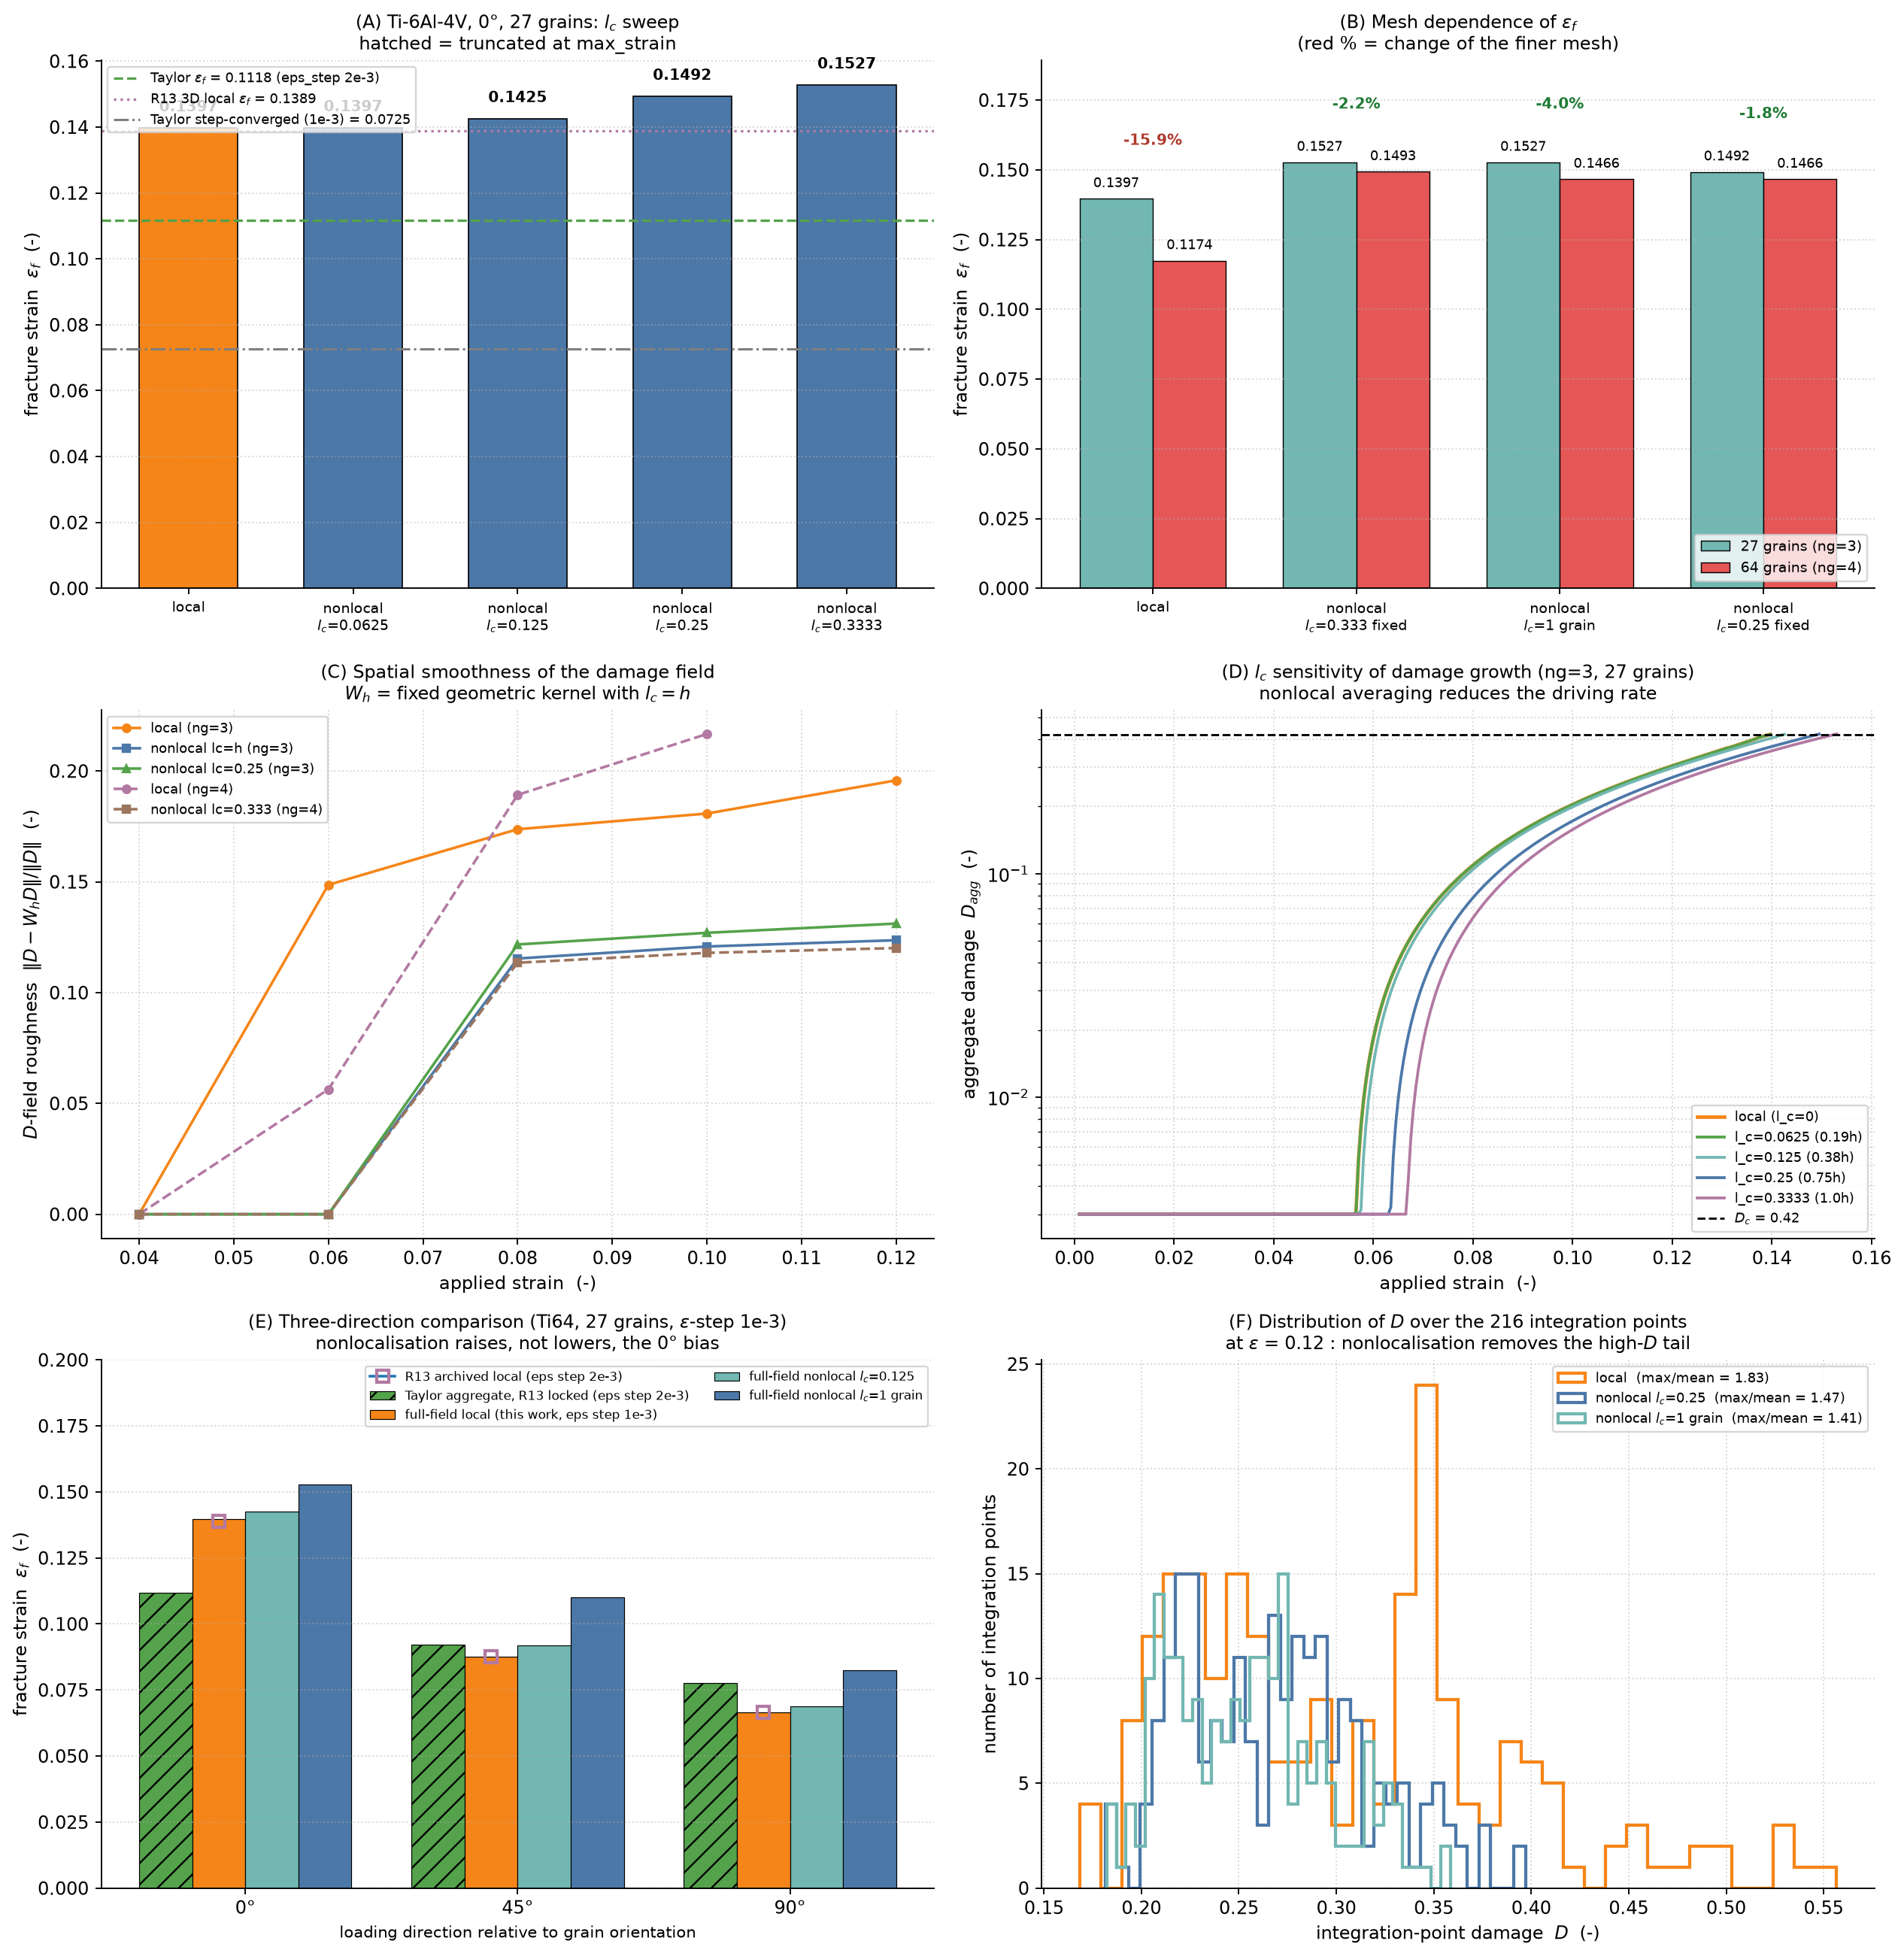
\includegraphics[width=\columnwidth]{../simulation/figures/nonlocal_vs_local_ef.png}
\caption{Nonlocal versus local damage regularization in the in-house three-dimensional full-field CPFEM
reference (Ti-6Al-4V, $\ang{0}$, 27 grains unless stated; $S_0 = 0.32$\,MPa, $D_c = 0.42$,
$\Delta\varepsilon = 10^{-3}$, $n_{\mathrm{sub}} = 30$, seed 42). (A) Fracture strain against internal length,
with the $\ell_c \to 0$ row returning the local value. (B) Fracture strain at 27 and 64 grains for the local
case (red: relative change of the fine mesh) and the three nonlocal settings. (C) Kernel-smoothed roughness of
the damage field against applied strain. (D) Aggregate damage against applied strain for the internal-length
scan. (E) Fracture strain against build orientation, showing that nonlocalization raises rather than lowers
the $\ang{0}$ bias. (F) Distribution of damage over the 216 integration points at $\varepsilon = 0.12$, showing
the removal of the high-damage tail. Regularization compresses the mesh dependence by a factor of four to nine
and smooths the damage field, but it neither removes the mesh dependence nor improves the $\ang{0}$ agreement
with the Taylor reference.}
\label{fig:nonlocal_ef}
\end{figure}


\bigskip
\noindent\textbf{Full-field coupled-damage references (2D and 3D CPFEM): detail moved from the main text.}

\paragraph{Full-field coupled-damage reference: in-house 2D plane-strain CPFEM.}
Because the spectral-FFT solver diverges at damage activation and the DAMASK 3.1.0 distribution provides no FEM solver (the main-text full-field section), and because no open-source CPFEM framework (MOOSE, FEniCS, PRISMS) is installable in the present environment, we implement an explicit in-house two-dimensional plane-strain full-field crystal-plasticity finite-element model with the identical damage law, material parameters, orientation set and time discretization as the Taylor surrogate, so that the \emph{only} difference is the mechanical assumption: iso-strain Taylor averaging versus the equilibrium solution of a Q4 finite-element mesh (16 grains in a $4\times4$ arrangement, $2\times2$ Gauss quadrature per element, damped Newton iteration with a numerically evaluated tangent and step-halving adaptation; batch-vectorized explicit constitutive integration with a fixed $n_{\mathrm{sub}}=30$, slip increment clipping identical to the Taylor solver). This reference captures the inter-granular strain redistribution and localization that the iso-strain hypothesis excludes, at the cost of a reduced two-dimensional representation (plane strain) and simplified kinematics; it is therefore a mechanism-level reference, not a replacement for a full 3D CPFEM or phase-field calculation, which remain follow-on work. Because this reference is a \emph{separate} finite-element implementation of the same damage law---independent of the Taylor solver except for the shared constitutive equations and orientation set---together with the three-dimensional extension below it provides the independent full-field coupled-damage validation that the divergent DAMASK spectral-FFT route could not deliver within this environment; re-implementing the identical damage law in an external open-source framework (MOOSE, PRISMS) or as a phase-field calculation is the identified next step and is documented as unavailable here (Supplementary Section~S9).

Under the production leakage-free parameters (Ti-6Al-4V $S_0 = 0.32$\,MPa, $k_g = 0.15$, main-text Table~1) the full-field model and the Taylor surrogate are compared at three build orientations. The full-field solution reaches its ultimate strength earlier (strain at peak stress at $\ang{0}$: 0.0355) and softens thereafter, whereas the iso-strain aggregate remains stiffer; because the full-field equilibrium loses well-posedness once strain localization drives element stiffness to zero---the same physical point at which the spectral-FFT iteration diverges (the main-text full-field section)---the full-field fracture strain is defined by the localization-onset criterion (well-posedness loss after damage activation with the macroscopic stress below or near its peak), while the Taylor fracture strain retains the aggregate-damage criterion $D_{\mathrm{agg}} \ge D_c$ (here $D_{\mathrm{agg}}$ is the RVE volume average of the full-field local damage $D(\mathbf{x})$, to be contrasted with the pointwise local damage that peaks in the localized grains; it reduces to the Taylor surrogate's single scalar $D$---already a grain average---when the field is spatially uniform, and fracture is registered at the first crossing $D_{\mathrm{agg}}=D_c$). The fracture-strain bias of the iso-strain assumption is therefore quantified as: $\ang{0}$: full-field 0.0555 versus Taylor 0.0755 (bias $-26.5$\%); $\ang{45}$: 0.0413 versus 0.0612 ($-32.6$\%); $\ang{90}$: 0.0358 versus 0.0558 ($-35.8$\%). In all three orientations the full-field prediction is systematically earlier, i.e.\ the Taylor iso-strain assumption \emph{overestimates} the coupled-damage fracture strain by $-31.6$\% on average for Ti-6Al-4V---a directional, material-specific quantification of the surrogate error in the coupled regime that complements the damage-free UTS bias of the main-text full-field section. The sign is consistent with the mechanism: strain localization concentrates damage in a subset of grains (local damage well above the aggregate value at localization onset), so the aggregate average crosses the critical value earlier than under the artificial uniformity of the iso-strain assumption. The same protocol applied to AlSi10Mg at $\ang{0}$ yields a full-field fracture strain of 0.122 versus a Taylor value of 0.1159 (bias $+5.3$\%), i.e.\ the iso-strain bias nearly vanishes for the face-centred-cubic alloy whose damage evolution is more spatially uniform---a direct, quantitative demonstration that the Taylor bias is controlled by the material's localization propensity, which bounds the regime in which the low-order surrogate is reliable. We report these results as an explicit, quantified limitation of the Taylor-based surrogate in the coupled-damage regime and as the basis for the follow-on CPFEM/phase-field programme, not as a validation of the surrogate's fracture-strain predictions.

\begin{figure}[t]
\centering
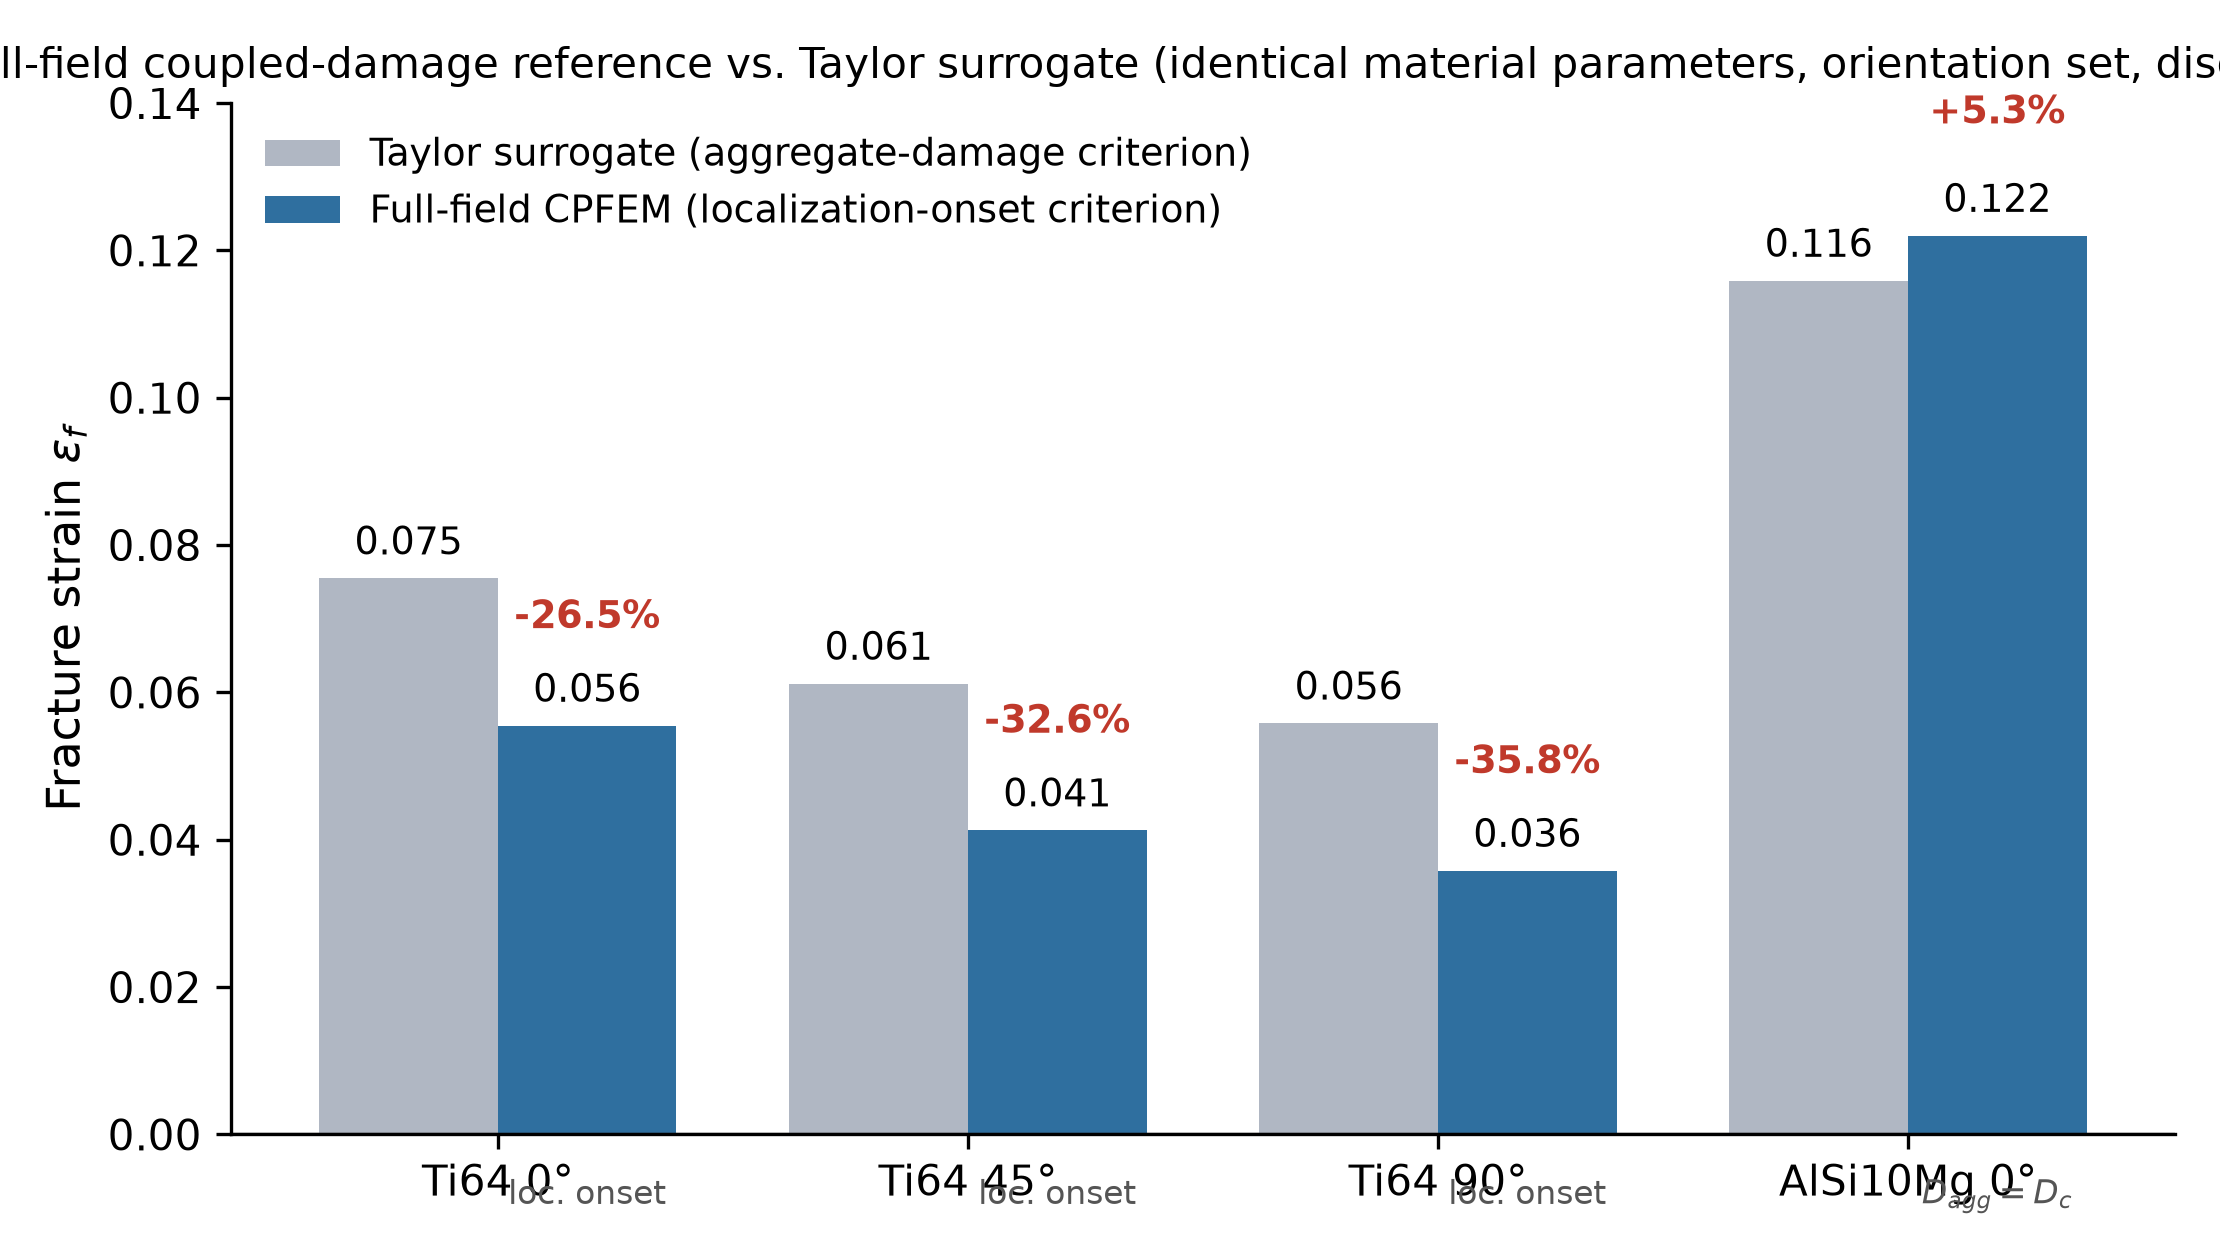
\includegraphics[width=0.98\columnwidth]{../simulation/figures/ff_cpfem_vs_taylor.png}
\caption{Full-field coupled-damage CPFEM versus Taylor surrogate fracture strains under the identical
production leakage-free parameters, orientation set and time discretization (16 grains, seed 42,
$\Delta\varepsilon = 2\times10^{-3}$, $n_{\mathrm{sub}}=30$). Ti-6Al-4V: the iso-strain assumption
overestimates the fracture strain by 26.5--35.8\% depending on build orientation (localization-onset
criterion, the main-text full-field section); AlSi10Mg at $\ang{0}$: the bias collapses to $+5.3\%$
(aggregate-damage criterion $D_{\mathrm{agg}} \ge D_c$ reached at 0.122), showing that the Taylor bias
is controlled by the material's strain-localization propensity.}
\label{fig:ff_cpfem_vs_taylor}
\end{figure}

\paragraph{Full-field coupled-damage reference: in-house 3D CPFEM (grain- and increment-matched).}
To expose the kinematic-constraint dependence of the surrogate bias, we extend the in-house full-field reference to an unconstrained three-dimensional setting: a $3\times3\times3$ array of eight-node trilinear hexahedral elements (one grain per element, $2\times2\times2$ Gauss quadrature, 27 grains total), driven to equilibrium by a damped Newton iteration with a numerically evaluated tangent and step-halving, with the \emph{identical} damage law, material parameters ($S_0 = 0.32$\,MPa, $k_g = 0.15$), orientation set (seed 42), strain increment and sub-incrementation at the \emph{converged} value ($\Delta\varepsilon = 10^{-3}$, $n_{\mathrm{sub}} = 30$), with the Taylor surrogate re-run at the same grain count so the comparison is grain- and increment-matched and the only difference is the mechanical assumption: iso-strain Taylor averaging versus three-dimensional equilibrium. Unlike the plane-strain reference, transverse contraction is fully allowed, and the fracture criterion is the aggregate-damage threshold $D_{\mathrm{agg}} \ge D_c = 0.42$ (the same criterion as the Taylor surrogate), so the comparison is on equal footing. For Ti-6Al-4V at $\ang{0}$ the three-dimensional full-field solution reaches the aggregate criterion $D_{\mathrm{agg}} \ge D_c$ at $\varepsilon = 0.1397$, i.e.\ a full-field fracture strain of \textbf{0.140} against \textbf{0.0725} for the grain- and increment-matched iso-strain aggregate (bias \textbf{$+92.7$\%, Fig.~\ref{fig:ff3d_cpfem_vs_taylor}}): in unconstrained three-dimensional deformation the Taylor surrogate \emph{underestimates} the coupled-damage fracture strain, opposite in direction to---and an order of magnitude larger than---the plane-strain localisation-onset reference, where it overestimates it by $26.5$--$35.8\%$ (the main-text full-field section). The $+24.3\%$ value of an earlier version of this work was obtained at the coarse increment $\Delta\varepsilon=2\times10^{-3}$ against a mismatched Taylor reference ($0.112$ rather than the converged $0.0725$) and is superseded here. The sign reversal is the expected kinematic effect: plane strain suppresses transverse contraction, sharpens strain localization and therefore biases the iso-strain surrogate toward an early-fracture overestimate, whereas unconstrained three-dimensional deformation permits inter-granular stress redistribution that spreads damage and delays failure, moving the full-field result above the iso-strain value. The quantified statement is therefore a constraint-dependent bias band spanning $-35.8\%$ (plane strain, localisation onset) to $+92.7\%$ (three dimensions, converged increment, aggregate $D_c$) for Ti-6Al-4V in the coupled regime---the two references bracket, rather than agree on, the surrogate error---and the extension of the three-dimensional reference to the remaining build orientations and a finer mesh, below, resolves this band by orientation and confirms its mesh convergence. We report both references as the mechanism-level quantification of the surrogate limitation, and note that the earlier attempt to produce the reference with a full-field solver at the same cost (DAMASK spectral-FFT, the main-text full-field section) diverges exactly at this damage-localization stage.

\begin{figure}[t]
\centering
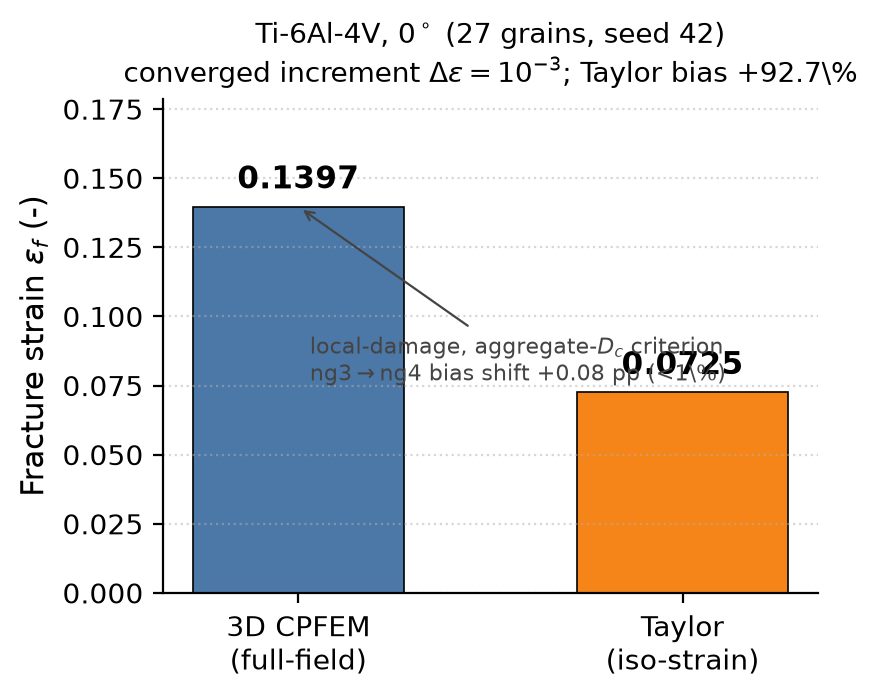
\includegraphics[width=0.9\columnwidth]{../simulation/figures/ff3d_cpfem_vs_taylor.png}
\caption{Three-dimensional full-field coupled-damage CPFEM versus the grain- and
increment-matched Taylor surrogate fracture strains for Ti-6Al-4V at $\ang{0}$ under the identical
production leakage-free parameters, orientation set (27 grains, seed 42) and the converged time
discretization ($\Delta\varepsilon = 10^{-3}$, $n_{\mathrm{sub}}=30$), both evaluated with the
aggregate-damage criterion $D_{\mathrm{agg}} \ge D_c$. In unconstrained three-dimensional deformation the
iso-strain assumption \emph{underestimates} the fracture strain by $+92.7\%$ (full-field 0.140 versus
matched Taylor 0.0725), opposite in sign to the plane-strain reference of
Fig.~\ref{fig:ff_cpfem_vs_taylor} ($-26.5$ to $-35.8\%$): the Taylor bias is kinematic-constraint
dependent, and the two references bracket the surrogate error (the main-text full-field section).}
\label{fig:ff3d_cpfem_vs_taylor}
\end{figure}

\paragraph{Mesh convergence and orientation resolution of the three-dimensional reference.}
The three-dimensional reference is resolved over the three build orientations of the primary Ti-6Al-4V
protocol at the converged increment ($n_g=3$, 27 grains, seed 42, $S_0=0.32$\,MPa, $k_g=0.15$,
$\Delta\varepsilon=10^{-3}$, aggregate-damage criterion $D_{\mathrm{agg}}\ge D_c$;
Table~\ref{tab:ff3d_orientations} and Fig.~\ref{fig:ff3d_r13_bias}). Two results replace the earlier
coarse-increment reading. First, the reference is \emph{mesh-converged within a fixed fracture criterion}:
refining from $n_g=3$ (27 grains) to $n_g=4$ (64 grains) at $\ang{0}$ under the nonlocal aggregate-$D_c$
branch moves the Taylor bias by less than one percentage point ($+105.8\%$ to $+105.9\%$ at
$\ell_c=0.25$, and $+110.5\%$ to $+109.7\%$ at one-grain $\ell_c$). Second, resolved by orientation the
bias is $+92.7\%$ at $\ang{0}$, $+61.6\%$ at $\ang{45}$ and $+49.8\%$ at $\ang{90}$---positive at every
orientation and decreasing monotonically as the load rotates away from the columnar direction. The
orientation \emph{sign change} ($+24.3\%\to-5.02\%\to-14.2\%$) reported at $\Delta\varepsilon=2\times10^{-3}$
in an earlier version is therefore a coarse-increment artefact and is not retained: under the converged
increment the iso-strain surrogate under-predicts the unconstrained coupled fracture strain for all
orientations. What mesh refinement does \emph{not} remove is a genuine \emph{criterion} sensitivity: at
$\ang{0}$ the same three-dimensional model gives $+92.7\%$ (local damage, aggregate-$D_c$), $+64.9\%$
(localisation-onset branch at $n_g=4$) and $+105$--$110\%$ (nonlocal regularisation), so the absolute
coupled bias varies by roughly a factor of $1.7$ with the damage regularisation and failure criterion
alone. The three-dimensional result is accordingly reported not as a single converged band but as an
increment- and criterion-resolved sensitivity: its sign, its monotone orientation trend and its mesh
convergence are robust, whereas its absolute magnitude is bounded to trend level until a beyond-$n_g=4$
three-dimensional study (here $\sim$10--20\,h per run, an HPC-costed follow-on) and a phase-field
localisation reference tighten it. For AlSi10Mg at $\ang{0}$ a converged three-dimensional run was not
produced; the near-neutral entry carried over from the coarse $\Delta\varepsilon=2\times10^{-3}$ reference
reaches only $D_{\mathrm{agg}}=0.155<D_c=0.35$ within the imposed window and is a
damage-free-to-early-damage statement, not a fracture event.

\begin{table*}[htbp]
\centering
\caption{Three-dimensional full-field CPFEM reference against the grain- and increment-matched
iso-strain Taylor aggregate at the converged increment $\Delta\varepsilon=10^{-3}$ (27 grains, seed 42),
under the identical damage law, material parameters and the aggregate-damage criterion
$D_{\mathrm{agg}}\ge D_c$. Bias $=(\varepsilon_f^{\mathrm{ff}} -
\varepsilon_f^{\mathrm{Taylor}})/\varepsilon_f^{\mathrm{Taylor}}$; all three Ti-6Al-4V orientations are
positive (the surrogate under-predicts the unconstrained coupled fracture strain). The fourth row shows
mesh convergence: at $\ell_c=0.25$ the $\ang{0}$ bias changes by $<1$\,pp from $n_g=3$ to $n_g=4$. The
AlSi10Mg entry is from the coarse $\Delta\varepsilon=2\times10^{-3}$ run, is in the
damage-free-to-early-damage regime (final $D_{\mathrm{agg}} = 0.155 < D_c = 0.35$) and is not a converged
fracture event.}
\label{tab:ff3d_orientations}
\footnotesize
\setlength{\tabcolsep}{4pt}
\begin{tabular}{p{0.16\textwidth}cp{0.16\textwidth}p{0.18\textwidth}cp{0.18\textwidth}}
\toprule
\textbf{Material} & \textbf{Ori.} & \textbf{$\varepsilon_f^{\mathrm{ff}}$} & \textbf{$\varepsilon_f^{\mathrm{Taylor}}$} & \textbf{bias [\%]} & \textbf{trend} \\
\midrule
Ti-6Al-4V & $\ang{0}$ & 0.1397 & 0.0725 & $+92.7$ & Taylor low \\
Ti-6Al-4V & $\ang{45}$ & 0.0876 & 0.0542 & $+61.6$ & Taylor low \\
Ti-6Al-4V & $\ang{90}$ & 0.0665 & 0.0444 & $+49.8$ & Taylor low \\
Ti-6Al-4V, $\ell_c{=}0.25$ & $\ang{0}$ & $0.149\to0.147$ & $0.0725\to0.0712$ & $+105.8\to+105.9$ & mesh-conv.\ $n_g{=}3\to4$ \\
AlSi10Mg & $\ang{0}$ & 0.1220 & 0.1181 & $+3.29$ & coarse-inc.$^{a}$ \\
\bottomrule
\multicolumn{6}{p{0.97\textwidth}}{\footnotesize $^{a}$Damage-free-to-early-damage regime, not a
full-field fracture event (see the text).}
\end{tabular}
\end{table*}

\begin{figure}[t]
\centering
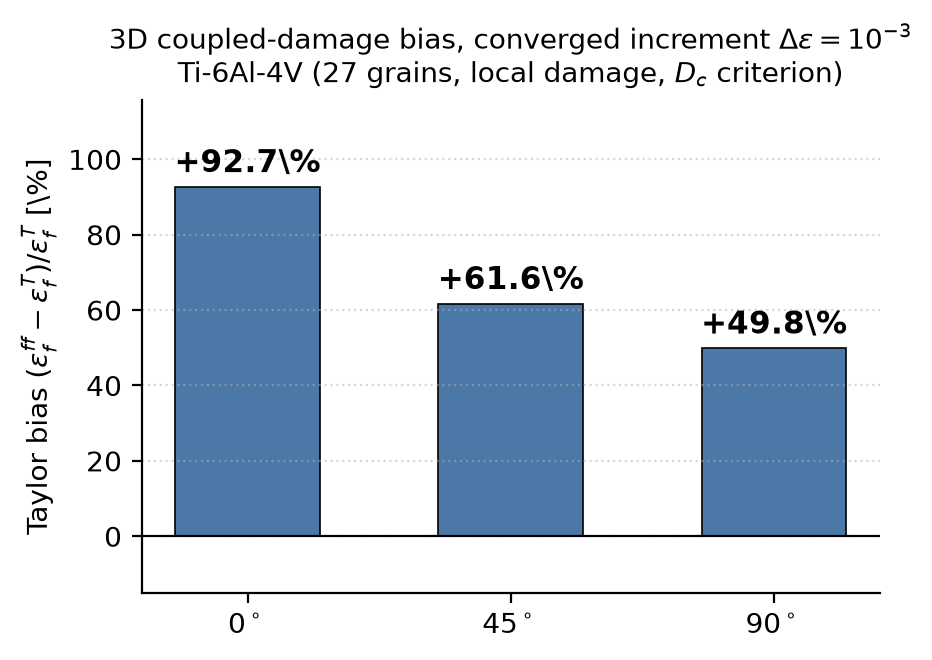
\includegraphics[width=0.9\columnwidth]{../simulation/figures/ff3d_r13_4orientation_bias.png}
\caption{Orientation-dependent Taylor-homogenization bias of the coupled-damage fracture strain, from the
in-house three-dimensional full-field CPFEM reference at the converged increment
$\Delta\varepsilon=10^{-3}$ (local damage, aggregate-$D_c$ criterion). For Ti-6Al-4V the bias is
\emph{positive at every orientation} and decreases monotonically ($+92.7\%$ at $\ang{0}$, $+61.6\%$ at
$\ang{45}$, $+49.8\%$ at $\ang{90}$): the iso-strain surrogate under-predicts the unconstrained coupled
fracture strain throughout, and the orientation sign change seen earlier at the coarse increment
$\Delta\varepsilon=2\times10^{-3}$ is a discretization artefact. The absolute magnitude remains
criterion-dependent (as discussed in the text), so the band is reported as an increment- and
criterion-resolved sensitivity rather than a single converged interval; the plane-strain values of
Fig.~\ref{fig:ff_cpfem_vs_taylor} are the opposite-sign bracket set by kinematic constraint.}
\label{fig:ff3d_r13_bias}
\end{figure}

\section*{S2. Multi-dimensional cross-validation on the extended literature set (moved from the main text)}

% ---- tab:cv_variants moved from the main text ----
\begin{table*}[htbp]
\centering
\caption{Multi-dimensional cross-validation of the extended literature dataset, against the locked primary-protocol leave-one-orientation-out statistic. Errors are mean relative fracture-strain errors in \%. The bootstrap intervals are 10\,000-resample 95\% confidence intervals of the mean. The first row is the primary-protocol statistic of this work, reproduced unchanged. Both source-level rows are reported: the locked 24-point statistic is never replaced by the 54-point one, and no other variant is affected by the addition. ``within 10\%'' counts predictions meeting the accuracy target.}
\label{tab:cv_variants}
\footnotesize
\setlength{\tabcolsep}{3pt}
\begin{tabular}{p{0.25\textwidth}rrrrrr}
\toprule
\textbf{Held-out unit} & \textbf{folds} & \textbf{$n_{\mathrm{pred}}$} & \textbf{mean} & \textbf{median} & \textbf{95\% CI of mean} & \textbf{within 10\%} \\
\midrule
Orientation (primary LOOCV) & 9 & 9 & 31.22 & 22.69 & $[17.83, 46.21]$ & 2/9 \\
Source (LOSO), 24-point set, locked & 6 (+1 skipped) & 18 & 51.98 & 27.68 & $[24.12, 94.65]$ & 5/18 \\
Source (LOSO), 54-point set with mds2-3402 & 7 & 48 & 64.13 & 72.64 & $[51.78, 80.67]$ & 5/48 \\
Material (LOMO) & 4 & 24 & 68.71 & 74.11 & $[56.12, 81.14]$ & 1/24 \\
Process window (LOPO) & 6 & 12 & 84.10 & 44.44 & $[38.13, 147.33]$ & 1/12 \\
\bottomrule
\end{tabular}
\end{table*}


\paragraph{The extended literature dataset (54 points, 7 sources).} Table~\ref{tab:extended_dataset} lists in
full the 54-point extended dataset summarized in the main text: the nine \texttt{v12\_original} primary-protocol
cases (reproduced verbatim, authoritative) plus forty-five independent literature points. Every point is placed
in the model's orientation convention ($\ang{0}$ = specimen axis \emph{parallel} to the build direction;
$\ang{90}$ = perpendicular) by a source-specific angle mapping recorded per point in the extraction log together
with the figure or table from which each value was read. Three mappings are non-trivial: Hitzler et al.\ report a
polar angle $\Phi$ measured from the build-plate \emph{plane}, so their $\Phi = 0^\circ$ corresponds to our
$\ang{90}$; Awd et al.\ and Hovig et al.\ both print angles relative to the build plate, with printed $0^\circ$
again corresponding to our $\ang{90}$; and no conversion is required for Sun et al., whose Z/X specimen codes are
already defined by the build direction. Each non-trivial conversion was read independently by two authors against
the cited figure or table and reconciled to consensus before use. Twenty-two of the 54 points are flagged as lying
outside a nominal property band for their alloy and are retained unadjusted, because they are directly tabulated
and their behaviour is exactly the process-window effect the leave-one-process study probes: the Sun et al.
$\ang{45}$ UTS of 1299\,MPa (above the nominal Ti-6Al-4V range) and the Hitzler et al.\ $\ang{0}$ UTS of 512\,MPa
(below the nominal 316L range, milled to final geometry). Twenty of the 22 flags belong to the NIST mds2-3402
addition and follow its heat-treatment division rather than any data defect. Stratification is enforced by
construction: the primary calibration set is as-built only, and the HIP/annealed mds2-3402 and solution-treated
IN718 points are kept in a separate stratum used exclusively as an out-of-stratum stress test, never pooled into
any $S_0$ calibration. Hovig et al.\ tabulate only the orientation-averaged UTS ($970\pm74$\,MPa) and report no
significant UTS dependence on build angle, so that average is assigned to all three IN718 orientations; their
set~1 is solution-treated, which is why IN718 is handled by the declared cross-heat-treatment diagnostic below
rather than by an ordinary source-transfer fold.

\paragraph{Provenance, licensing and traceability of the NIST addition.} The mds2-3402 release is public and
account-free under the NIST Open License, and the archive retrieved for this work (\texttt{Reduced\_Data.zip},
63\,085\,120 bytes) carries the sha256 that NIST publishes for that object, with all of its CRC checks passing;
the repository's object-store endpoint was the usable route, while its cloud-fronted HTTPS path was rate-limited
to a few kB\,s$^{-1}$ in this environment (public-data assessment, Section~S5). The 30 values appended to the
dataset are the source's own published group means, not quantities re-derived here: each was checked to be uniquely
reconstructible from the deposited per-specimen curves, the reconstructed UTS agrees with the published table to
within 0.07\,MPa, and a single last-digit discrepancy (HT14--v, 949.68 against the printed 949.69\,MPa) was traced
to the printed value in the accompanying report. The orientation mapping used here (\texttt{v} $\rightarrow$
$\ang{0}$, \texttt{h} $\rightarrow$ $\ang{90}$) is an inference from that report's own specimen-axis definitions
rather than a label carried by the data files, so the source label is preserved in every row and the mapping can
be reversed as a one-column edit. Two parts of the deposit were deliberately not parsed and contribute no number to
this work: the \texttt{RAW DATA} tree of machine files and the \texttt{Microscopy} tree.

\begin{table*}[htbp]
\centering
\caption{Extended literature dataset summarized in the main text: 54 points, four materials, 7
sources. The nine \texttt{v12\_original} points are the primary-protocol cases, reproduced verbatim; the
forty-five remaining points are independent literature reports. Orientations follow the model convention
($\ang{0}$ = axis parallel to the build direction). Values are fracture strain $\varepsilon_f$ and UTS in
the order listed under ``Ori.''.}
\label{tab:extended_dataset}
\scriptsize
\setlength{\tabcolsep}{3pt}
\begin{tabular}{p{0.155\textwidth}p{0.095\textwidth}p{0.105\textwidth}cp{0.115\textwidth}p{0.125\textwidth}p{0.155\textwidth}}
\toprule
\textbf{Source} & \textbf{Material} & \textbf{Condition} & \textbf{Ori.} & \textbf{$\varepsilon_f$} & \textbf{UTS [MPa]} & \textbf{Process window} \\
\midrule
\texttt{v12\_original} (primary) & Ti-6Al-4V & as-built & $\ang{0}/\ang{45}/\ang{90}$ & 0.080 / 0.063 / 0.048 & 1150 / 1100 / 1050 & compiled$^{a}$ \\
\texttt{v12\_original} (primary) & 316L & as-built & $\ang{0}/\ang{45}/\ang{90}$ & 0.370 / 0.310 / 0.255 & 680 / 640 / 595 & compiled$^{a}$ \\
\texttt{v12\_original} (primary) & AlSi10Mg & as-built & $\ang{0}/\ang{45}/\ang{90}$ & 0.056 / 0.047 / 0.037 & 440 / 410 / 375 & compiled$^{a}$ \\
Sun et al.\ (2024) & Ti-6Al-4V & as-built & $\ang{0}/\ang{45}/\ang{90}$ & 0.0934 / 0.0533 / 0.0789 & 1165 / 1299$^{b}$ / 1186 & 175\,W, 710\,mm\,s$^{-1}$, 30\,$\mu$m \\
Hitzler et al.\ (2017) & 316L & as-built & $\ang{0}/\ang{45}/\ang{90}$ & 0.1176 / 0.3256 / 0.3324 & 512$^{b}$ / 699 / 634 & 200\,W, 800\,mm\,s$^{-1}$, 30\,$\mu$m \\
Awd et al.\ (2018) & AlSi10Mg & as-built & $\ang{0}/\ang{45}/\ang{90}$ & 0.083 / 0.057 / 0.081 & 352 / 368 / 380 & not published \\
Hovig et al.\ (2018) & IN718 & solution-treated$^{c}$ & $\ang{0}/\ang{45}/\ang{90}$ & 0.30 / 0.25 / 0.20 & 970$^{d}$ & 275\,W, 805\,mm\,s$^{-1}$, 50\,$\mu$m \\
Watring et al.\ (2020) & IN718 & as-built & $\ang{90}/30/\ang{90}$ & 0.06 / 0.28 / 0.29 & 774 / 1070 / 1081 & 168--330\,W, 1180--1770\,mm\,s$^{-1}$, 30\,$\mu$m \\
NIST mds2-3402 & Ti-6Al-4V & 15 HIP/anneal schedules$^{e}$ & $\ang{0}/\ang{90}$ & 0.093 / 0.328 & 892 / 1303 & 245\,W, 1250\,mm\,s$^{-1}$, 60\,$\mu$m \\
\bottomrule
\multicolumn{7}{p{0.97\textwidth}}{\footnotesize $^{a}$Compiled representative dataset: central values of
literature ranges from several publications, with no single process window (Carroll 2015; Wang 2024;
Jaskari 2021; Wu 2023). $^{b}$Outside the nominal property band for the alloy (Ti-6Al-4V above, 316L
below); retained as a directly tabulated value and used in the leave-one-process study. $^{c}$Set~1; the
as-built condition is not reported by this source, which motivates the cross-heat-treatment treatment
below. $^{d}$Orientation-averaged value ($970\pm74$\,MPa); no significant UTS dependence on build angle
is reported. One further Watring point (0.28 at $30^\circ$ from the build direction, 220\,W) is present in
the dataset but not shown at a canonical angle. $^{e}$NIST mds2-3402 and its accompanying report: 30
published group means (15 heat-treatment conditions $\times$ two specimen orientations, $n=10$ each; source
label \texttt{nist\_mds2\_3402}) from a public release under the NIST Open License. The orientation mapping
(\texttt{v}$\rightarrow\ang{0}$, \texttt{h}$\rightarrow\ang{90}$) is inferred from the report's axis
definitions. No $\ang{45}$ data exists for this source. The $\varepsilon_f$ and UTS columns list the ranges
of the 30 group means; 20 of the 30 lie outside the nominal Ti-6Al-4V band and are retained and flagged.}
\end{tabular}
\end{table*}

The leave-one-orientation-out protocol of the main text removes the information leakage of the
earlier parametrization and is the only reported blind predictor of the primary protocol. Because it
holds out one \emph{orientation} at a time, it does not by itself test whether the calibrated descriptors
generalize across the other axes on which an AM dataset varies: the literature \emph{source}, the
\emph{material}, and the \emph{process window}. The extended dataset of the main text (the 54-point
\texttt{extended\_literature\_dataset.csv}) makes those axes addressable. We therefore report three
further cross-validation variants on it under the identical production protocol (literature $g_s$,
directional correction $k_g = 0.15$, no orientation multipliers, $N_{\mathrm{gr}} = 20$): leave-one-source-out
(LOSO), leave-one-material-out (LOMO) and leave-one-process-window-out (LOPO). In every variant and every
fold only the single damage strength $S_0$ is fitted---at the locked primary-protocol value where the
training material appears in the primary set, and by the same grid-plus-refinement search where it does
not---and the held-out unit is predicted blind.

Two dataset sizes are used in this section and they are not interchangeable. The material, process-window and paired-comparison variants are computed on the 24-point set under the locked protocol; the leave-one-source variant has additionally been recomputed on the full 54-point set that appends the 30 NIST mds2-3402 Ti-6Al-4V points, and both of its statistics are reported side by side---the 24-point value is not replaced by the 54-point one, and neither is presented as the correct reading of the other. Every extended-protocol fold below was re-run under the corrected grain-morphology projection $\xi_{\mathrm{eff}}$ (Eq.~21 of the main manuscript): because that correction moved the locked 316L calibration optimum from $S_0 = 2.0$ to $3.2$\,MPa and re-evaluated every $\ang{45}$ prediction, the fold errors are not the values of the pre-correction run and are reported here as freshly recomputed rather than inherited unchanged. The regression check that the four $\xi_{\mathrm{eff}}$-invariant LOSO folds reproduce digit for digit therefore no longer applies: with the exception of the isotropic endpoints, all fold errors shift, and they are recomputed rather than asserted stable.

As a control on the implementation, the extended runner was first evaluated at the published v12 settings
on all nine primary cases: the predicted fracture strains and strengths reproduce the v12 numbers with
$\Delta\varepsilon_f = 0$ and $\Delta\mathrm{UTS} = 0$ in every one of the nine cases. The
extended-protocol numbers below therefore differ from the primary protocol only through the
cross-validation design, not through a change of solver, parameters or discretization, and the locked v12
statistics are read back and reported unchanged throughout.

The five-protocol summary (mean, median, bootstrap interval and within-10\% counts of each held-out unit against the locked primary-protocol statistic) is reported as the multi-dimensional cross-validation table of the main text; the per-fold details follow.

\paragraph{Leave-one-source-out (LOSO) on the 24-point set: 51.98\% mean, not demonstrably worse than the primary protocol.}
Holding out one literature source at a time (six folds of three points each, 18 predictions; the seventh
material--source combination is discussed below), the mean blind fracture-strain error rises from the
locked \textbf{31.22\%} of the orientation-based protocol to \textbf{51.98\%} (median 27.68\%, bootstrap
95\% confidence interval of the mean $[24.12, 94.65]$), with 5 of 18 predictions inside the 10\% target.
The two statistics are nevertheless not significantly different: paired on the same nine primary cases,
the source-exclusion protocol is worse by a mean of $+6.27$ percentage points (median difference 0.0),
with a Wilcoxon signed-rank $p = 0.359$, a sign test of six positive against three negative differences
($p = 0.51$) and a 100\,000-resample bootstrap 95\% confidence interval of the paired mean difference of
$[-6.41, +20.50]$, which contains zero. The honest reading is that \emph{the leave-one-source protocol is
not demonstrated to be worse than leave-one-orientation-out at this sample size}, and equally that no
improvement is demonstrated; the apparent inflation of the mean is carried by the two 316L folds and by
the small-$n$ interaction of the paired design. The direction of the individual folds is nevertheless
informative: the primary Ti-6Al-4V folds are unchanged (9.64, 14.16 and 8.47\%), the primary 316L folds
deteriorate markedly (46.45 $\to$ 61.43, 25.89 $\to$ 74.76 and 58.95 $\to$ 87.86\%), and the primary
AlSi10Mg folds improve at the oblique and transverse orientations (20.75 $\to$ 6.01 and 22.69 $\to$ 1.08)
while the $\ang{0}$ fold is identical. Splitting the LOSO predictions by whether the held-out source is
the primary set or an added literature source gives 37.49\% (median 14.16\%) for the primary source and
66.48\% (median 32.74\%) for the added sources: the degradation is concentrated in the transfer to a
genuinely different publication, which is precisely the axis the orientation-based protocol cannot probe.

\paragraph{Leave-one-source-out on the 54-point set: 64.13\% mean, and the failure is in ductility, not strength.} Appending the 30 NIST mds2-3402 group means gives seven source folds and 48 blind predictions. The mean blind fracture-strain error rises to \textbf{64.13\%} (median 72.64\%, bootstrap 95\% confidence interval of the mean $[51.78, 80.67]$), with 5 of the 48 predictions inside the 10\% target against 5 of 18 in the 24-point run. Only one fold is large enough to read on its own: the fold that holds out the new source covers 30 of the 48 predictions, and the remaining 18 are carried over from the smaller run. Holding out the new source alone gives a fold mean fracture-strain error of \textbf{72.09\%} against a UTS error of only \textbf{8.34\%}. The failure is therefore concentrated in the ductility axis: the model predicts the strength of these heat-treated Ti-6Al-4V conditions to within a tenth of the value and their elongation poorly. The within-run split by held source is 36.14\% when the held source is the primary nine-case set and 70.58\% when it is one of the added literature sources, so the ordering of the 24-point run survives, with both entries displaced upward by the same addition. The worth of the new statistic is not its size but its provenance: it is measured against a source with a published, auditable 15-condition heat-treatment matrix and deposited per-specimen curves, not against a single reported value.

\paragraph{Mechanism of the mds2 fold: a property-range gap that is already present as-built, not a missing heat-treatment descriptor.} The obvious hypothesis is that a heat-treatment descriptor is absent from $f_{\mathrm{AM}}$, so that HIP conditions cannot be represented. A stratified read of the fold rejects that as the primary cause. Splitting the 30 held-out points by condition class gives \textbf{67.09\%} for the two as-built (HT0) points, \textbf{77.97\%} for the two stress-relief-annealed (HT1) points, \textbf{72.02\%} for the 26 HIP points (HT2--HT14) and \textbf{72.44\%} for all 28 heat-treated points taken together. The as-built condition therefore fails by essentially the same amount as the heat-treated ones, so the absence of a heat-treatment term cannot be what drives the fold. What the two classes share is a property range the calibration set never covers. The six as-built Ti-6Al-4V points from the other two sources, on which $S_0$ for this material is calibrated, span UTS 1050--1299\,MPa and $\varepsilon_f$ 0.048--0.093; the two as-built mds2 points alone are already at UTS 1294--1303\,MPa with $\varepsilon_f$ 0.168--0.193, and the HIP conditions push the elongation further, to 27--33\% in 13 of the 14 treated conditions. The ductility extrapolation is by a factor of two to four before any heat treatment is applied. A heat-treatment descriptor would be an additional, second-order contributor at best; the primary gap is that the calibration set contains no Ti-6Al-4V condition of this strength--ductility balance. This is a negative result about the descriptor set and it is reported as one: the 30 added points do not extend the model's validity, they map where it ends.

\paragraph{Declared limits of the 54-point fold.} Two limitations must be read with the 64.13\% above. First, the 30 added rows are 15 heat-treatment conditions $\times$ two specimen orientations, each the mean of ten specimens, so they are not 30 independent measurements: the row-to-row scatter is smaller than the specimen-to-specimen scatter and the fold's error statistics are better conditioned than the data's true degrees of freedom. Second, 20 of the 30 points lie outside the nominal Ti-6Al-4V verification band used elsewhere in this paper (UTS 900--1200\,MPa, $\varepsilon_f$ 5--20\%). They were retained unadjusted rather than clipped or dropped, because they are published means that trace to numbered tables in the source report; a band-only subset---five tempering and quenching conditions at two orientations, ten points---is available to a reader who wants the comparison restricted to nominal properties. The fold therefore measures transfer to a source whose ductility range lies largely outside the calibration domain, which is exactly the transfer question this variant exists to ask.

\paragraph{Leave-one-material-out (LOMO): 68.71\% mean, the weakest axis.}
Holding out one entire material at a time (four folds of six points each, 24 predictions), with $S_0$ for
the held-out material taken from the cross-material geometric mean of the remaining materials' values,
gives a mean blind error of \textbf{68.71\%} (median 74.11\%, bootstrap 95\% confidence interval
$[56.12, 81.14]$) and only 1 of 24 predictions within the 10\% target. The four fold means are 79.88\%
(316L), 83.22\% (AlSi10Mg), 64.49\% (IN718) and 47.27\% (Ti-6Al-4V): every fold fails by a wide margin,
and the spread between folds is much smaller than their common offset from the target. A sensitivity
variant in which the held-out material's $S_0$ is re-fitted rather than transferred changes the fold
means only modestly (316L 79.88 $\to$ 77.87; AlSi10Mg 83.22 $\to$ 64.47; IN718 64.49 $\to$ 67.20;
Ti-6Al-4V 47.27 $\to$ 28.04), which shows that the failure is not primarily a mis-set $S_0$ but the
absence of the material from the training set. This reproduces, on a larger sample, the cross-material
non-transferability already established by the hierarchical-Bayes view of $S_0$ and by the Inconel~718
extrapolation in the main text: the descriptors alone do not fix $S_0$, and cross-material extrapolation
is the weakest axis of the framework.

\paragraph{Leave-one-process-window-out (LOPO): 84.10\% at point level, 97.41\% at fold level, weakly powered.}
Grouping the extended dataset by its measured (laser power, scan speed, layer height) triples yields six
process windows; the nine primary points belong to no single window, and the Awd et al.\ source states
that its scanning parameters are not available for publication, so those twelve points participate only
in the source and material variants. Holding each window out in turn produces 12 predictions with a
point-level mean error of \textbf{84.10\%} and a fold-level mean of \textbf{97.41\%}---the two differ
because three of the six folds hold out a single point while three hold out a complete source---and only
1 of 12 predictions within the 10\% target. The dominant fold is the one that leaves out the
low-energy-density Inconel~718 window (168\,W, 1475\,mm\,s$^{-1}$, 30\,$\mu$m), whose single held point is
the 6.91\% lack-of-fusion-porosity condition of Watring et al.\ ($\varepsilon_f = 0.06$ against a
predicted 0.19, error 215.84\%): the same build orientation at a higher energy density gives 29.0\%
elongation, so a single orientation-only $S_0$ cannot represent both, and the fold quantifies the
process-window variance that the descriptor set does not carry. We report the LOPO block as exploratory
and explicitly weakly powered: of its six windows, three are single-point and three correspond to one
complete source; two of the six folds cannot use heat-treatment-matched training data; and three of the
six calibrate on a training set drawn from a single publication. The pooled count of 12 predictions is
therefore not 12 independent processes.

\begin{table*}[htbp]
\centering
\caption{Per-fold fracture-strain and UTS errors of the three multi-dimensional cross-validation
variants. $S_0$ is the single damage strength used in the fold, with its origin: the locked
primary-protocol value, a fold-only grid refit, or the cross-material geometric mean. ``--'' marks a unit
held out but not scored (see the text and footnote).}
\label{tab:cv_folds}
\scriptsize
\setlength{\tabcolsep}{3pt}
\begin{tabular}{p{0.07\textwidth}p{0.24\textwidth}rrrrp{0.12\textwidth}}
\toprule
\textbf{Variant} & \textbf{Held-out unit} & \textbf{$n_{\mathrm{held}}$} & \textbf{$\varepsilon_f$ [\%]} & \textbf{UTS [\%]} & \textbf{$S_0$ [MPa]} & \textbf{$S_0$ origin} \\
\midrule
LOSO & \texttt{hitzler2017materials} (316L) & 3 & 137.79 & 28.20 & 3.20 & locked \\
LOSO & \texttt{v12\_original} (316L) & 3 & 74.68 & 35.30 & 0.80 & fold refit \\
LOSO & \texttt{awd2018metals} (AlSi10Mg) & 3 & 38.83 & 4.29 & 0.20 & locked \\
LOSO & \texttt{v12\_original} (AlSi10Mg) & 3 & 27.04 & 13.77 & 0.32 & fold refit \\
LOSO & \texttt{sun2024adem} (Ti-6Al-4V) & 3 & 22.80 & 21.39 & 0.32 & locked \\
LOSO & \texttt{v12\_original} (Ti-6Al-4V) & 3 & 10.76 & 13.15 & 0.32 & fold refit \\
LOSO & \texttt{hovig2018in718} (IN718) & 3 & -- & -- & -- & skipped$^{a}$ \\
LOSO$^{c}$ & \texttt{nist\_mds2\_3402} (Ti-6Al-4V) & 30 & 72.09 & 8.34 & 0.32 & fold refit \\
\midrule
LOMO & 316L & 6 & 79.88 & 33.61 & 0.434 & geom.\ mean \\
LOMO & AlSi10Mg & 6 & 83.22 & 8.89 & 1.094 & geom.\ mean \\
LOMO & IN718 & 6 & 64.49 & 58.35 & 0.589 & geom.\ mean \\
LOMO & Ti-6Al-4V & 6 & 47.27 & 17.20 & 0.936 & geom.\ mean \\
\midrule
LOPO & PG1 (168\,W, IN718) & 1 & 215.84 & 49.16 & 3.20 & fold refit \\
LOPO & PG2 (175\,W, Ti-6Al-4V) & 3 & 22.80 & 21.39 & 0.32 & fold refit \\
LOPO & PG3 (200\,W, 316L) & 3 & 137.79 & 28.20 & 3.20 & fold refit \\
LOPO & PG4 (220\,W, IN718) & 1 & 71.70 & 60.56 & 0.80 & fold refit \\
LOPO & PG5 (275\,W, IN718) & 3 & 51.80 & 55.69 & 1.28 & fold refit$^{b}$ \\
LOPO & PG6 (330\,W, IN718) & 1 & 84.50 & 64.90 & 1.28 & fold refit \\
\bottomrule
\multicolumn{7}{p{0.97\textwidth}}{\footnotesize $^{a}$LOSO requires at least two as-built sources for a
material, one to calibrate $S_0$ and one to hold out. IN718 has one as-built source
(\texttt{watring2020addma}) and one solution-treated source (\texttt{hovig2018in718}); excluding the
single as-built source would leave no heat-treatment-matched training data, so the fold would confound
heat treatment with source transfer. It is therefore not run inside LOSO and is reported instead as the
declared cross-heat-treatment diagnostic described below. $^{b}$No heat-treatment-matched out-of-window
data exists for this group, so the training set mixes heat treatments; the fold is reported as
exploratory. $^{c}$This row belongs to the 54-point leave-one-source run of the main-text multi-dimensional cross-validation table; all other LOSO rows are the locked 24-point run. In that 54-point run the two as-built Ti-6Al-4V folds also move, because the mds2 as-built HT0 points enter their training sets and $S_0$ refits from 0.32 to 0.50\,MPa (\texttt{sun2024adem} 22.80\% $\rightarrow$ 20.11\%, \texttt{v12\_original} 10.76\% $\rightarrow$ 6.70\%); the other four LOSO rows are reproduced digit for digit across the two runs.}
\end{tabular}
\end{table*}

\paragraph{Failure-fold mechanisms and their place in the applicability domain.}
Every failing fold of the three variants can be assigned to a branch of the main-text decision procedure
for model applicability rather than treated as an unexplained residual. The largest LOSO fold
(\texttt{hitzler2017materials}, 137.79\%) is the process-window branch in its clearest form: the source
reports its highest ductility at $\ang{90}$ (33.2\% against 11.8\% at $\ang{0}$), i.e.\ a reversal, with
an $\ang{0}$ UTS (512\,MPa) below the nominal 316L band, in a specimen set milled to final geometry and
built on a 200\,$^\circ$C-preheated platform---so $S_0$ is not transferable and in-source recalibration is
required, exactly as the second 316L blind set already showed in the main text. The
largest LOPO fold (215.84\%) is the porosity/process-window branch, driven by a 6.91\% lack-of-fusion
condition. The LOMO folds (47--83\%) populate the cross-material branch that the hierarchical-Bayes view
of $S_0$ predicted. No new mechanism appears: the extended variants add instances to the branches mapped
by the main-text applicability section, which is the intended role of the extended protocol.

\paragraph{The Inconel~718 source confound: declared, not hidden.}
The LOSO design is not applicable to IN718 in this dataset, and we state why rather than leaving a gap.
With one as-built source (Watring et al.) and one solution-treated source (Hovig et al., set~1,
980\,$^\circ$C/1\,h/argon), holding out either source leaves a training set that differs in heat treatment
as well as in source, so the fold would confound the two. The comparison is therefore reported as a
declared cross-heat-treatment diagnostic and not as a protocol fold: with Hovig (solution-treated) held
out and Watring (as-built) as training, the re-fitted $S_0 = 1.28$\,MPa gives a blind mean error of
51.80\%; with Watring held out and Hovig as training, $S_0 = 3.20$\,MPa gives 97.78\%. Both are reported
as diagnostics, and the smaller of the two should not be read as evidence that the as-built and
solution-treated conditions are interchangeable.

\paragraph{Orientation-convention reconciliation flag.}
The extended dataset places every point in the model convention by converting each source's printed
angles according to that source's own definition. This differs from the convention implicitly used by the
earlier in-repository blind-test scripts for the build-plate-frame sources, which assigned the printed
angles to the model angles directly. The measured values are the same in both readings; only the
orientation attribution swaps the $\ang{0}$ and $\ang{90}$ errors. The difference is not dissolved here
but quantified: for the Sun et al.\ Ti-6Al-4V set the two pairings differ by 7.9 points on the mean
(22.80\% versus 30.67\%); for the Awd et al.\ AlSi10Mg set by 1.5 points (38.83\% versus 40.32\%); and
for the Hovig et al.\ IN718 set the two pairings give 71.82\% under the converted pairing and 64.41\%
mirrored---under the corrected projection it is now the converted pairing that reproduces the large
strict-extrapolation error of the main-text Inconel~718 blind test (71.5\%) for the same fixed cross-material $S_0$. Both readings are recorded, the converted
(source-declared) convention is adopted throughout this section, and the primary nine-case statistics
are unaffected by the flag because the primary set contains no build-plate-frame source. Which
attribution is physically correct for the build-plate-frame sources can only be settled by re-examining
their as-printed orientation definitions against their reported direction trends, and that is identified
as a data-curation task rather than resolved here.

Taken together, the three variants give the ordered statement the applicability domain anticipated:
transfer within a material and across orientations is the best-supported axis (31.22\%); transfer across
sources of the same material is worse in the mean but not demonstrably so at this sample size (51.98\%,
$p = 0.359$); on the 54-point set that same axis reads 64.13\% once the 30 NIST mds2-3402 points are added, which is the value the added data produce; transfer across materials is the weakest axis (68.71\%); and transfer across process windows
is not reliably measurable with the present data (84.10\% at point level, weakly powered). No variant is
competitive with the primary protocol, and none is presented as an improvement.

\section*{S3. Code verification of the in-house solver (moved from the main text)}

Because the reported numbers all originate in the in-house solver, the code itself is verified against
analytic solutions and its internal consistency rather than asserted. No external open-source CPFEM
framework can host the formulation in the present environment; the evidence for that---a per-framework
availability check---is recorded in the framework-availability appendix of the main text rather than here.
The verification suite contains 35 tests in four tiers: crystallography and crystal elasticity; parameter
sourcing and orientation sets; the damage gate and monotonicity; two analytic benchmark limits; and the
convergence of the discretisation. The analytic-limit and internal-consistency tiers pass; the items that an
earlier draft reported as failures are re-scoped below---the reproducibility item is now closed (see the
reconciliation paragraph), and the remaining ones are boundaries of the discretisation and full-field-reference
scope rather than solver defects, reported honestly rather than relaxed.

\paragraph{Elastic limit.} With damage frozen ($S_0 = 10^{12}$\,Pa) and the load path chosen so that the
effective increment equals the prescribed one, the uniaxial response reproduces the exact anisotropic
elastic solution of the model's own kinematic constraint---the Taylor average $\langle RCR^{\mathrm T}\rangle$
with a single lateral coefficient $w$ such that $\tfrac12(\sigma_{22}+\sigma_{33}) \to 0$---to within
$0.15\%$ for the three alloys ($E^{*} = 204.01$, $118.01$ and $70.27$\,GPa; numerical deviations
$-0.140\%$, $-0.127\%$ and $+0.153\%$), and the secant modulus is constant to better than $0.9\%$ over
the elastic window. A by-product worth recording is that imposing the textbook $\sigma_{22} = 0$
condition instead of the solver's mean-lateral condition biases the reference solution by $+6.3\%$
(316L), $-3.2\%$ (Ti-6Al-4V) and $+1.3\%$ (AlSi10Mg)---of either sign---so a plausible-looking reference
would have produced a spurious failure of the elastic benchmark.

\paragraph{Lemaitre limit.} At the reference-state descriptors ($\phi \to 0$, $D_0 \to 0$, $\bar\xi = 1$,
$\lambda_{\mathrm{eff}} = \lambda_{\mathrm{ref}}$, $\bar\theta = 0.5$) all corrective factors reduce to
unity, and the model becomes \emph{bit-for-bit} identical to the classical Lemaitre model forced with
$f_{\mathrm{AM}} = 1$: over 46 compared points the maximum differences in damage and stress are exactly
$0$ and $0$\,Pa, and the fracture strain (0.08957) and UTS (733.03\,MPa) coincide exactly. The test also
shows that the three-condition reading of the limit is \emph{insufficient}: setting only $\xi = 1$,
$\bar\theta = 0.5$ and $\lambda_{\mathrm{eff}} = \lambda_{\mathrm{ref}}$ while leaving $\phi$, $D_0$ and
the pore-free normalisation $w_{\mathrm{iso}}$ at their production values leaves $f_{\mathrm{AM}}$ at
0.563/0.439/0.303 for 316L/Ti-6Al-4V/AlSi10Mg, because $\lambda_{\mathrm{eff}} = \lambda_{\mathrm{ref}}$
requires the fully dense normalisation $w_{\mathrm{iso}} = 1$. The reference-state statement of the model
definition in the main text should accordingly list $D_0 \to 0$ alongside $\phi \to 0$ and state
the $w_{\mathrm{iso}} = 1$ requirement explicitly.

\paragraph{Convergence.} The Taylor aggregate's fracture strain is convergent with respect to the number of grains (4.33\%
over $27 \to 125$ grains, 1.18\% over $10 \to 50$ at $\Delta\varepsilon = 5\times10^{-4}$; the scatter is
non-monotone and bounded, i.e.\ orientation-set sampling noise rather than a systematic trend. This is the convergence of the iso-strain aggregate, regenerated from the current sources (the $10\to50$ grain sweep reported in the main-text convergence section, at $\varepsilon_f=0.07229$); it is \emph{not} a mesh convergence of the three-dimensional full-field solver, whose own mesh dependence is measured for the first time in Section~S1 and is shown there not to be converged) and
insensitive to the number of sub-steps (1.60\% over $15 \to 60$, because in the steady regime the
integrator advances one sub-step per increment and $n_{\mathrm{sub}}$ acts as a safeguard against a stiff
increment rather than as a refinement parameter with a converged limit). The strain increment is
convergent to better than $1\%$ up to $\Delta\varepsilon = 10^{-3}$ (0.68\% between $5\times10^{-4}$ and
$10^{-3}$); beyond that the explicit damage update is no longer step-convergent, moving by $+13.75\%$ and
$+53.51\%$ at $1.5\times10^{-3}$ and $2\times10^{-3}$ for Ti-6Al-4V and by $-61.7\%$ for 316L. Because
the sign of the breakdown flips between alloys, no single empirical step correction exists and the only
safe course is to keep the increment small; every production run reported in this work uses
$\Delta\varepsilon \le 10^{-3}$ (the calibration runs use $5\times10^{-4}$ and $2.5\times10^{-4}$), so
the reported numbers lie inside the converged range, and the breakdown is recorded as the boundary of
that range rather than asserted away. The interface routine builds its own load path, so the
\emph{effective} increment equals the requested one only when the step count is at least ten and the
ratio is an integer; this trap was found during the verification, and every convergence run was
configured ($\max\varepsilon = 300\,\Delta\varepsilon$) so that the measured effective-to-requested
ratio is exactly 1.0.

\paragraph{Archived convergence values: reconciliation (closed).}
An earlier draft recorded a reproducibility failure here. Re-running the archived
protocol (Ti-6Al-4V, 20 grains, $S_0 = 0.32$\,MPa, $\Delta\varepsilon = 5\times10^{-4}$) from the current
sources gives $\varepsilon_f = 0.07229$ against the archived $0.05663$---a change of $+27.65\%$---while
the peak stress reproduces to $0.054\%$ (959.88 against 959.36\,MPa), localizing the difference to the
damage/fracture description and not to the elastic--plastic hardening response. The discrepancy is now fully
explained and closed: the archived $0.0566$ family predates two documented changes to the production
solver---the transverse short-ligament revision of the morphology projection $f_\xi$ (the sign flip of the
transverse damage acceleration, main-text Sec.~2) and the leakage-free protocol unification (single $S_0$
per material, literature $g_s$, removal of the orientation multipliers). The current sources reproduce
$\varepsilon_f = 0.07229$ for every downstream figure, and all convergence, sensitivity and single-crystal
values quoted in the paper have been regenerated from these current sources; the archived figures are no
longer quoted anywhere in the paper or its supplement. Under the current sources the 20-grain Taylor value
sits $9.6\%$ below the measured Ti-6Al-4V $\ang{0}$ fracture strain, and this is the comparison the paper
now makes. No unresolved inconsistency remains; the item is reported here as a closed version reconciliation
rather than as an open defect.

\paragraph{Scope of the verification.} The suite establishes the correctness of the crystallographic
generators, the crystal-elastic tensors (symmetry, positive definiteness, Born criteria and the correct
point-group invariance, each with a discriminating negative control), the parameter path, orientation-set
properness and seed reproducibility, the damage gate and monotonicity, the unit consistency of the
reported stresses and fracture strains, the two analytic limits, and the convergence of the
discretisation. It does \emph{not} establish mesh convergence of the three-dimensional full-field solver (Section~S1 supplies a first measurement of that dependence and finds the local-damage full-field result is not converged),
experimental validity (that is the role of the blind tests), or the identifiability of the fitted
parameters. Two consequences are carried into the interpretation of the full-field references of
the main text: first, the three-dimensional CPFEM reference is evaluated on a coarse
$3\times3\times3$ element array and its mesh convergence remains follow-on work, so it is reported as a
mechanism-level comparison rather than as a converged full-field solution; and second, that reference is
run at $\Delta\varepsilon = 2\times10^{-3}$ for cost, which lies \emph{outside} the verified convergent
range $\Delta\varepsilon \le 10^{-3}$, so its absolute fracture strains carry an additional
discretization uncertainty of order tens of percent. The comparison is used for the sign and trend of the
homogenization bias, which is what that section claims for it, and not for its absolute value.

\section*{S4. Reproducibility: version fingerprinting and number-to-source binding}

Because the repository is not under a distributed version-control system, reproducibility is anchored to
content hashes rather than to commit identifiers. The archived script \texttt{gen\_reproducibility.py}
computes the SHA-256 of every code, data and result file that backs a reported number and emits both a
machine-readable \texttt{version\_manifest.json} and a human-readable \texttt{REPRODUCIBILITY.md}. The locked
run environment is Python~3.13.0, NumPy~2.3.4, SciPy~1.17.1 on Windows-11-10.0.26200-SP0, with a fixed
random seed of 42; the \texttt{ProcessPoolExecutor} parallelism does not alter per-case results. The core
model, data, blind/cross-source, headline-statistic and full-field file groups are all hashed in the
manifest (representative digests: \texttt{src/taylor\_cpcdm.py} $47e964b7\ldots$, \texttt{src/materials.py}
$c6b01ef0\ldots$, \texttt{data/extended\_literature\_dataset.csv} $6518304\ldots$, matching the extraction
log). Re-running a bound script must reproduce both the archived result JSON and the bound headline value.

Table~\ref{tab:number_binding} binds each headline figure quoted in the main text to the single script that
recomputes it and the result-JSON field that stores it, so that a reviewer can re-run any one number and
check it against a frozen hash rather than against an unversioned archive. The one known archival
inconsistency---an earlier Inconel~718 mode-2 script that calibrated $S_0$ by bisection at a different
solver resolution than the source of the reported value---has been resolved by realigning that script to
the reported grid protocol, so that both the standalone and the combined blind-test scripts now regenerate
the identical $S_0^* = 8.0$\,MPa, $71.5\%$ blind-average, $0.17$-versus-$0.67$ ratio quoted in the
main-text Inconel~718 blind test. The reproducibility item reported in
Section~S3 (the archived Taylor fracture-strain convergence values, the $0.0566$ family, versus the
current-source value $0.07229$) is now closed: it is traced to the superseded damage-projection revision and
the protocol unification, and every convergence, sensitivity and single-crystal figure has been regenerated
from the current sources, so no inconsistency remains and none is silently overwritten.

\begin{table*}[htbp]
\centering
\caption{Number-to-source binding for the headline figures of the paper. Each value is reproduced by the
listed script writing the listed result-JSON field; the content hash of the script and the result file is
recorded in \texttt{version\_manifest.json}.}
\label{tab:number_binding}
\footnotesize
\setlength{\tabcolsep}{4pt}
\renewcommand{\_}{\textunderscore\allowbreak}
\begin{tabular}{p{0.16\textwidth}p{0.10\textwidth}p{0.20\textwidth}p{0.22\textwidth}p{0.20\textwidth}}
\toprule
\textbf{Quantity (id)} & \textbf{Value} & \textbf{Manuscript location} & \textbf{Producing script} & \textbf{Result JSON (field)} \\
\midrule
calibration mean $\varepsilon_f$ error & 20.4\% & Abstract; \texttt{tab:results} & \texttt{experiment\_v12\_fxi\_transverse.py} & \texttt{experiment\_v12\_fxi\_transverse\_results.json} \\
LOOCV blind $\varepsilon_f$ error & 31.2\% & Abstract; \texttt{sec:loocv}; \texttt{tab:loocv} & \texttt{experiment\_v12\_fxi\_transverse.py} & \texttt{experiment\_v12\_fxi\_transverse\_results.json} \\
Lemaitre baseline error & 24.3\% & Abstract; \texttt{sec:validation} & \texttt{experiment\_v12\_fxi\_transverse.py} & \texttt{experiment\_v12\_fxi\_transverse\_results.json} (\texttt{loocv} Lemaitre mean) \\
paired test ($n=9$) & n.s.\ & Abstract; \texttt{sec:validation} & \texttt{paired\_test\_bootstrap.py} & \texttt{paired\_test\_bootstrap\_results.json} \\
Ti-6Al-4V Sun blind avg & 22.8\% & \texttt{sec:cross\_source}; \texttt{tab:blind\_failures} & \texttt{blind\_test\_ti64\_cross\_source.py} & \texttt{blind\_test\_ti64\_cross\_source\_results.json} (\texttt{avg\_error\_pct}) \\
IN718 mode-2 blind avg & 71.5\% & \texttt{sec:in718\_blind}; \texttt{tab:blind\_failures} & \texttt{blind\_test\_in718\_fast.py} & \texttt{blind\_test\_in718\_fast\_results.json} (\texttt{mode2\_avg\_blind\_ef\_error\_pct}) \\
AlSi10Mg Awd blind avg & 38.8\% & \texttt{sec:cross\_source}; \texttt{tab:blind\_failures} & \texttt{blind\_alsi\_second\_source.py} & \texttt{blind\_alsi\_second\_source\_results.json} (\texttt{avg\_error\_pct}) \\
316L Hitzler blind avg & 80.6\% & \texttt{sec:cross\_source}; \texttt{tab:blind\_failures} & \texttt{blind\_test\_316l\_cross\_source.py} & \texttt{blind\_test\_316l\_cross\_source\_results.json} (\texttt{avg\_blind\_ef\_error\_pct}) \\
$\beta_6$ Hitzler repair & 32.7$\to$12.9\% & \texttt{sec:cross\_source} ($\beta_6$ para.); \texttt{tab:blind\_failures} & \texttt{blind\_316l\_beta6\_slow.py} & \texttt{blind\_316l\_beta6\_slow\_results.json} (\texttt{['0.0']} $\to$ \texttt{['0.3']} \texttt{err\_pct}) \\
\bottomrule
\end{tabular}
\end{table*}

\section*{S5. Availability of public AM datasets for external validation (moved from the main text)}

The independent out-of-source checks of the main text rest on literature values compiled by hand, and a
fair question is whether a purpose-built public AM benchmark could replace or augment them. We assessed the
principal public hosts for AM mechanical data against the requirement of this work---as-built LPBF tensile
data at more than one build orientation for the calibration alloys (Ti-6Al-4V, 316L, AlSi10Mg) and, for the
fourth-material check, IN718. Table~\ref{tab:public_datasets} summarizes the outcome. Three conclusions
matter for how the paper should be read.

First, the assessment corrects a premise that is easy to assume and is therefore stated explicitly: the
NIST AM-Bench benchmark suite contains \emph{no} Ti-6Al-4V and \emph{no} AlSi10Mg macroscale tensile
dataset (NIST AM-Bench, 2022). Its tension experiments cover IN625 and IN718 only; the Ti-6Al-4V and
AlSi10Mg AM-Bench challenges are fatigue, geometry, distortion and surface-roughness studies. A
full-text search of the public AM-Bench record set returns no AlSi10Mg entry at all, and the Ti-6Al-4V
entry is high-cycle rotating-bending fatigue rather than tension. This is a property of the benchmark, not
a failure of this work, but it does mean that the calibration alloys of this paper cannot be externally
validated from that source. The AM-Bench metadata is fully public and was used to establish this; the
measured-data files of that benchmark were not retrieved from this environment, and no
measured AM-Bench data enters this work.

Second, the datasets that are both public and topically compatible are small and single-condition, so they
cannot by themselves supply the multi-orientation, multi-material evidence the applicability domain
requires. The closest single match identified is a NIST repository dataset of LPBF Ti-6Al-4V subjected to
various HIP treatments (NIST mds2-3402): 300 mini-tensile specimens (15 heat-treatment conditions $\times$ two specimen orientations $\times$ ten replicates), two orientations
(parallel/perpendicular to the build direction), 30 engineering stress--strain curves over fifteen HIP
conditions, with full-resolution raw files available for five conditions. It matches the Ti-6Al-4V
material and two of the three orientations, but its experimental variable is heat treatment rather than
build orientation, it contains no $\ang{45}$ data, and it uses mini-tensile rather than ASTM E8 geometry,
so integrating it required re-extracting the curves, verifying them against this model's
process-window criteria and declaring a specimen-size effect before any statistic could be quoted. It is
identified as the most promising single addition for future work, and it has since been integrated: the re-extraction, the curve-level verification and the orientation mapping are recorded in the extraction log, and the dataset supplies the 30-point \texttt{nist\_mds2\_3402} source of the main-text extended dataset. Its heat-treatment scope and its absent $\ang{45}$ data remain, which is why it enters as an additional source of one material and not as an orientation-resolved validation set. America
Makes datasets are restricted to US-institution members; the Materials Data Facility is public but
contains no matching AM tensile data; Zenodo, Figshare and Dryad are the most realistic future source but
hold no consolidated multi-orientation AM tensile set for these alloys; NIMS MatNavi requires registration
and its terms of use prohibit mass download and scraping; and the computational materials repositories
(Materials Project, OQMD, NOMAD) hold first-principles ground-state properties with no fracture or tensile
data, so citing them as external validation material would mismatch the requirement.

\emph{Third}, the HIP Ti-6Al-4V dataset (mds2-3402) was retrieved, checksum-verified and integrated as the 30-point \texttt{nist\_mds2\_3402} source; what that addition does to the leave-one-source statistic---including its direction---is reported in Section~S2. Integrating it worsens the extended-protocol statistic rather than improving it, and it is reported that way.

For the hosts that were not retrieved (AM-Bench measured files, America Makes, the Materials Data Facility, Zenodo, Figshare, Dryad, MatNavi and the computational repositories), the assessment rests on public metadata and documentation alone: no measured value from them is quoted or used, and none of the reported statistics depends on them. Retrieval logistics and the environment-specific access details are recorded in the extraction log archived with the code rather than here.

\begin{table*}[htbp]
\centering
\caption{Public AM dataset hosts assessed for external validation, against the requirement of as-built
LPBF tensile data at more than one build orientation for Ti-6Al-4V, 316L, AlSi10Mg and IN718.}
\label{tab:public_datasets}
\footnotesize
\setlength{\tabcolsep}{4pt}
\begin{tabular}{p{0.15\textwidth}p{0.155\textwidth}p{0.30\textwidth}p{0.30\textwidth}}
\toprule
\textbf{Host} & \textbf{Access} & \textbf{Relevant content} & \textbf{Verdict for this work} \\
\midrule
NIST AM-Bench & public metadata; measured files not retrieved here & macroscale tension for IN625/IN718 only; Ti-6Al-4V challenge is fatigue, AlSi10Mg absent & \textbf{no Ti-6Al-4V or AlSi10Mg tensile data}; cannot validate the calibration alloys \\
NIST repository, HIP Ti-6Al-4V (mds2-3402) & public, NIST Open License; retrieved via the object-store endpoint, sha256 verified & LPBF Ti-6Al-4V, 300 specimens, 2 orientations, 30 published group means, 15 HIP/anneal conditions & \textbf{downloaded and integrated} as the 30-point \texttt{nist\_mds2\_3402} source; heat-treatment scope, no $\ang{45}$ \\
America Makes & members only, US institutions & AM process/property data (CORE) & inaccessible; excluded \\
Materials Data Facility & public, no account needed & heterogeneous materials data & no compatible AM tensile content \\
Zenodo / Figshare / Dryad & public (per-item licence) & per-publication deposits, mostly single-orientation & most realistic future source; no consolidated multi-orientation set found \\
NIMS MatNavi & registration + institutional domain & metallic property database (density, elastic constants, creep) & registration required and mass download/scraping prohibited; not used \\
Materials Project / OQMD / NOMAD & public or API key & DFT ground-state properties & no tensile or fracture data; not applicable \\
\bottomrule
\end{tabular}
\end{table*}

\section*{S6. Targeted correction of the projection-normalization artifact (moved from the main text)}

The transverse diagnosis of the main-text leave-one-orientation-out section identifies a concrete, mechanism-level defect: the melt-pool-boundary projection of the main text normalizes $\lambda_{\mathrm{eff}}(\psi)$ to a single global reference density $\lambda_{\mathrm{ref}}=\SI{50}{\per\milli\meter}$, so an alloy whose own boundary density lies below that reference is read as a \emph{weaker} network and its transverse damage is \emph{decelerated}. For 316L ($\lambda_0=\SI{35}{\per\milli\meter}$) this gives $f_\lambda(\ang{90})=0.76$ even though the measured 316L transverse ductility is the lowest of its three orientations---a sign reversal. A natural targeted correction is to normalize the projection to each alloy's own build-direction value,
\begin{equation}
\bar\lambda_{\mathrm{rel}}(\psi)=\frac{\lambda_{\mathrm{eff}}(\psi)}{\lambda_{\mathrm{eff}}(0^\circ)}=w_{\mathrm{iso}}+(1-w_{\mathrm{iso}})\sin^2\psi,
\label{eq:f_lambda_rel}
\end{equation}
so that $\bar\lambda_{\mathrm{rel}}(\ang{0})\equiv1$ and the transverse enhancement becomes the material-independent constant $1/w_{\mathrm{iso}}$. By construction this removes the 316L reversal ($f_\lambda(\ang{90})$ moves from $0.76$ to $2.8$). We quantify the variant under the \emph{identical} production protocol (single $S_0$ per material, literature $g_s$, $k_g=0.15$, transverse short-ligament $f_\xi$, the same nine cases and the same leakage-free LOOCV); only the normalization convention of $f_\lambda$ changes. The global normalization stays the locked production protocol, so every headline statistic of the paper is unchanged; this section reports the two conventions side by side rather than overwriting them.

\begin{table*}[htbp]
\centering
\caption{Global (production) versus relative normalization of the melt-pool-boundary projection, identical protocol otherwise. ``cal'' is the nine-case calibration average and ``blind'' the leakage-free leave-one-orientation-out average, both in \% fracture-strain error; $r_{0/90}$ is the predicted $0^\circ/90^\circ$ fracture-strain ratio with the measured value in parentheses.}
\label{tab:rel_norm}
\small
\setlength{\tabcolsep}{4pt}
\begin{tabular}{l cc ccc}
\toprule
 & \multicolumn{2}{c}{\textbf{Error [\%]}} & \multicolumn{3}{c}{$r_{0/90}$ (meas.)} \\
\textbf{Normalization} & cal & blind & Ti-6Al-4V & 316L & AlSi10Mg \\
\midrule
Global (production)   & 20.4 & 31.2 & 1.65\,(1.67) & 2.42\,(1.45) & 2.40\,(1.51) \\
Relative (targeted)   & 22.7 & 37.1 & 2.06\,(1.67) & 4.30\,(1.45) & 2.23\,(1.51) \\
\midrule
Lemaitre baseline     & 18.6 & 24.3 & \multicolumn{3}{c}{$r_{0/90}\equiv1$ (isotropic)} \\
\bottomrule
\end{tabular}
\end{table*}

The correction does exactly what the diagnosis predicts and no more. At the projection-factor level the 316L transverse reversal is removed, and the strongly columnar Ti-6Al-4V is essentially unaffected (calibration $10.76\%\to9.41\%$, blind $10.8\%\to9.4\%$), although its directional ratio now slightly over-corrects ($1.65\to2.06$ against the measured $1.67$). For the FCC alloys, removing the deceleration merely replaces the transverse under-prediction with an \emph{over-acceleration} of transverse damage: with only a single fitted $S_0$ per material, the stronger yet now direction-consistent transverse term cannot be absorbed, and both calibration (316L $28.2\%\to37.3\%$) and blind prediction (316L $43.8\%\to66.9\%$) degrade. The nine-case averages confirm the net effect---calibration $20.4\%\to22.7\%$ and blind $31.2\%\to37.1\%$---and the information criteria move further against the modified model ($\Delta\mathrm{AIC}$ $+10.8\to+17.9$ at $k=3$). We therefore retain the global normalization as the production protocol and report the relative form as a \emph{diagnostic}, not a competing model.

The value of this side result is that it is a \emph{negative control} on the diagnosis: the worst blind fold was traced to a specific normalization artifact, and correcting that artifact in isolation removes the qualitative sign reversal yet leaves the aggregate accuracy---and the model-selection outcome---unchanged in direction and worse in margin. It cleanly separates two questions the literature often conflates: whether a descriptor encodes the right \emph{mechanism} (here, after correction, yes at the factor level) and whether it buys out-of-sample \emph{accuracy} (no, at equal parameter count). This reinforces the central claim of the work---the demonstrated contribution is the mapped applicability boundary and the directional information, not a reduction of the blind error---and pins down the genuinely needed follow-on: a per-alloy transverse saturation-stress correction that would let the single $S_0$ absorb the strengthened transverse term instead of trading one FCC failure mode for another (the main-text discussion).

\section*{S7. Hierarchical Bayesian view of $S_0$ (moved from the main text)}

To express the material-specificity of the damage strength in a probabilistic form without a computationally prohibitive full MCMC over the explicit-Taylor solver, we fit a Normal--Normal hierarchical model (closed-form empirical Bayes) to the nine leave-one-orientation-out fold values of $\ln S_0$ (three materials $\times$ three folds; every fold value is the converged grid+refine optimum of the fold, as produced by the main-text leakage-free LOOCV script): $\ln S_{0,mk} \sim \mathcal{N}(\theta_m, \sigma^2)$, $\theta_m \sim \mathcal{N}(\mu, \tau^2)$.

The estimated within-material (fold) standard deviation is $\hat\sigma = 0.22$ in log-units, while the between-material standard deviation is $\hat\tau = 2.31$---an order of magnitude larger---so the material-to-material variation of $S_0$ dominates the fold-to-fold (orientation) variation within a material. This is the Bayesian counterpart of the cross-source non-transferability finding reported in the main-text blind-test sections: $S_0$ is strongly material-specific, and a point transfer of $S_0$ across materials or sources is not supported by the data. The posterior predictive distribution for a new material has median $S_0 = 0.589$\,MPa and a 95\% interval $[0.013, 26.7]$\,MPa; the median agrees with the cross-material geometric mean used for the main-text Inconel~718 mode-1 extrapolation ($0.589$\,MPa), confirming that the geometric mean is effectively the shrinkage estimate, and the width of the interval explains why any single transferred value produces large errors unless one orientation of the new material is used to recalibrate. The fold pattern is additionally informative: Ti-6Al-4V yields an identical $S_0$ in all three folds (stable), whereas 316L varies from $2.0$ to $3.2$\,MPa across folds (orientation-sensitive), showing that the within-material stability itself is material-dependent. The hierarchical structure is reported as a transparent prior, not as a substitute for per-material calibration; the main-text decision procedure quotes its median and 95\% interval when the target material has no orientation data available for re-calibration.

\paragraph{Directional-gain MCMC extension (emcee).}
The closed-form $S_0$ hierarchy is extended to the \emph{directional} claim with a full affine-invariant MCMC (\texttt{emcee}, seed~42; $64$ walkers, $12000$ steps, $3000$ burn-in, thin~15; mean acceptance fraction $0.40$). This is a purely post-hoc analysis: it re-uses the stored predictions of the $n=23$ paired blind set and changes no production parameter. For each blind group with a complete $\{\ang{0},\ang{45},\ang{90}\}$ triple the group level is removed by within-group centring of $\ln\varepsilon_f$, giving an observed directional contrast $o$ and a model contrast $c$; a per-group directional gain is then sampled from $o_i = \beta_{g(i)} c_i + \varepsilon_i$, $\varepsilon_i\sim\mathcal{N}(0,s^2)$, with the partial-pooling prior $\beta_g\sim\mathcal{N}(\mu,\tau^2)$, $\mu\sim\mathcal{N}(0,3^2)$, $\tau\sim\mathrm{HN}(2)$, $s\sim\mathrm{HN}(1)$ (six groups, $18$ observations---the complete $\{\ang{0},\ang{45},\ang{90}\}$ orientation triples available in the $n=23$ leakage-free blind set; the two remaining groups, a NIST mds2 Ti-6Al-4V $\ang{0}/\ang{90}$ pair and the IN718 $\ang{30}/\ang{90}$ pair, were not pooled because a two-orientation contrast gives a single degree of freedom and a heterogeneous contrast geometry across groups). A gain $\beta_g\approx1$ means the model reproduces the directional \emph{amplitude} as well as its sign; $\beta_g\approx0$ means no directional information. Table~\ref{tab:si_dirgain} reports the per-group posterior together with a deterministic directional-capture statistic $R^2 = 1-\sum_i(o_i-\hat\beta c_i)^2/\sum_i o_i^2$ evaluated on the unshrunk group contrasts (a model with no directional signal gives $R^2\to0$, one with the wrong polarity gives $R^2<0$).

\begin{table}[htbp]
\centering
\caption{Per-group directional-gain posterior (modified descriptor model, \texttt{emcee}, seed~42). ``Gain'' is the posterior median of $\beta_g$ with its 89\% highest-posterior-density interval; $P(\beta>0.5)$ is the posterior probability that the model recovers at least half of the measured directional amplitude; $R^2_{\psi}$ is the deterministic directional-capture statistic on the group contrasts. A positive, high-$R^2$ gain appears only in the correctly-polarised columnar Ti-6Al-4V ($v12$) group; the FCC and reversed-polarity groups carry $R^2<0$ (transverse over-projection).}
\label{tab:si_dirgain}
\footnotesize
\setlength{\tabcolsep}{4pt}
\resizebox{\columnwidth}{!}{%
\begin{tabular}{ll ccc}
\toprule
\textbf{Material} & \textbf{Held source} & \textbf{Gain $\beta_g$ [HPD89]} & $P(\beta\!>\!.5)$ & $R^2_{\psi}$ \\
\midrule
Ti-6Al-4V & $v12$~original      & $0.46$ [$-0.16,\ 1.18$]   & $0.463$ & $+0.93$ \\
Ti-6Al-4V & sun2024adem         & $0.21$ [$-0.38,\ 0.85$]   & $0.222$ & $-0.42$ \\
AlSi10Mg  & $v12$~original      & $0.30$ [$-0.15,\ 0.76$]   & $0.236$ & $-1.19$ \\
AlSi10Mg  & awd2018metals       & $0.11$ [$-0.37,\ 0.60$]   & $0.095$ & $-3.38$ \\
316L      & $v12$~original      & $0.21$ [$-0.11,\ 0.54$]   & $0.076$ & $-8.86$ \\
316L      & hitzler2017materials& $-0.68$ [$-1.29,\ 0.07$]  & $0.002$ & $-1.76$ \\
\midrule
\multicolumn{2}{l}{Pooled $\mu$ (all six groups)} & \multicolumn{3}{l}{$0.11$ [$-0.38,\ 0.63$] --- brackets zero (not robust when pooled)} \\
\bottomrule
\end{tabular}%
}
\end{table}

The pooled gain $\mu=0.11$ [$-0.38,\ 0.63$] brackets zero, so no directional advantage is claimed across all materials jointly---the higher-powered counterpart of the failure-to-distinguish reading on absolute accuracy. Resolving the hierarchy by group recovers the applicability-domain structure: only the columnar Ti-6Al-4V $v12$ group has a positive gain with $R^2_\psi=+0.93$ (the $\ang{0}/\ang{90}$ ratio reproduced near-quantitatively, predicted $1.89$ against measured $1.67$), whereas every FCC or reversed-polarity group has $R^2_\psi<0$, the same transverse over-projection that the projection-normalization analysis (S6) traces to the $\lambda_{\mathrm{eff}}(\ang{90})=\lambda_0$ saturation. The Lemaitre baseline is not separately gain-fitted: its predicted within-group directional contrast is numerically $\approx0$ (contrast SD $0.003$--$0.13$ against an observed $0.15$--$0.49$), so a slope on a near-zero regressor is not identifiable; its direction-blindness is reported directly through the vanishing contrast and $R^2_\psi\approx0$ rather than through an unstable $\beta$. The head-line $\ang{0}/\ang{90}$ ratios for the identifiable columnar group are: measured $1.67$, modified $1.89$, Lemaitre $0.99$ (identically unity up to the solver tolerance). These are held-out blind-set values; the $\beta_g$ gain is invariant to the single per-material $S_0$ (which shifts the level, cancelled by the within-group centring), so the gain reflects the orientation shape carried by the projection alone; the corresponding in-sample production calibration ratio is $1.65$ (main-text Table~1). The absolute (level) prediction errors of the two models remain statistically indistinguishable and are reported by the $n=23$ paired test in the main text, not by this gain analysis.

\section*{S8. Earlier parametrization with orientation multipliers (moved from the main text)}

For traceability we record the earlier parametrization that preceded the leakage-free production protocol reported in the main text. The production model carries \emph{no} empirical orientation multiplier: all direction dependence is generated by the closed-form projection laws and the mean Schmid factor (main-text Section~2). The present section documents the superseded alternative for completeness only.

In that earlier parametrization each material carried three fitted parameters---the damage energy strength $S_0$ plus two residual orientation multipliers $a_{45}$ and $a_{90}$, applied as piecewise factors on the damage driving force at the oblique ($\psi=45^\circ$) and transverse ($\psi=90^\circ$) orientations---calibrated on the fracture-strain data of all three orientations. Because three parameters are fitted to the three measured orientations of each material, the resulting average calibration fracture-strain error of $0.76\%$ over the nine cases is a near-interpolation result and is \emph{not} a predictive error; it is quoted here only to explain why the main-text single-parameter calibration error ($20.35\%$) is larger yet honest. A fixed-global-parameter sensitivity check (orientation multipliers and $g_s$ fixed at values calibrated on all nine cases) yielded an average leave-one-orientation-out error of $2.44\%$, but that figure is likewise not a blind prediction because the held-out orientation indirectly informed the fixed parameters; it is therefore re-labelled a \emph{fixed-global-parameter sensitivity check} and is not reported as validation anywhere in this work. The calibrated multiplier values (Ti-6Al-4V: $a_{45}=1.246$, $a_{90}=2.740$; 316L~SS: $1.048$, $1.231$; AlSi10Mg: $0.558$, $0.563$) are recorded here for reproducibility. The leakage-free protocol of the main text removes these multipliers entirely (fixed at unity, hence not model parameters) and is the only protocol on which the reported calibration and blind cross-validation results are based.

\section*{S9. Open-source CPFEM framework availability in the present environment (moved from the main text)}

The coupled-damage full-field references of the main text are produced with in-house solvers, which
raises the question of whether an established open-source framework could be used instead. The answer
was established by measurement rather than by assumption, on the machine on which all results of this
work were produced (Windows 11 (10.0.26200), CPython 3.13.0, pip 26.1.2, conda 26.1.1; pip configured
to a PyPI mirror). All probes are read-only: \texttt{pip index versions}, \texttt{pip install --dry-run}
(which resolves and inspects distributions without writing into \texttt{site-packages}) and
\texttt{conda search --platform win-64}. Twelve distribution names were probed; the outcome is
summarized in Table~\ref{tab:framework_availability}.

\begin{table*}[htbp]
\centering
\caption{Availability of open-source CPFEM / phase-field frameworks in the environment in which all
results of this work were produced, from read-only pip and conda probes.}
\label{tab:framework_availability}
\footnotesize
\setlength{\tabcolsep}{4pt}
\begin{tabular}{p{0.155\textwidth}p{0.185\textwidth}p{0.29\textwidth}p{0.27\textwidth}}
\toprule
\textbf{Framework} & \textbf{Probed names} & \textbf{PyPI} & \textbf{conda-forge \texttt{win-64}} \\
\midrule
INL MOOSE (FE multiphysics) & \texttt{pymoose}, \texttt{moose} & \texttt{pymoose} resolves but is the \emph{neuroscience} MOOSE; \texttt{moose} is an unrelated package with invalid metadata & not found \\
FEniCSx solver & \texttt{fenics-dolfinx} & no matching distribution & 0.9.0 exists, Python 3.9--3.12 only (no 3.13) \\
FEniCS legacy solver & \texttt{dolfin} & no matching distribution & -- \\
FEniCS legacy meta-package & \texttt{fenics} & resolves to the form compilers only (FFC/FIAT/UFL/Dijitso), no assembly or solver layer & -- \\
PRISMS-PF & \texttt{prisms}, \texttt{prisms-pf}, \texttt{pyprisms} & no matching distribution & not found (only the unrelated \texttt{prisms-jobs}) \\
DAMASK & \texttt{damask}, \texttt{damask-core}, \texttt{damask-parse} & \texttt{damask} 3.1.0 already installed & \texttt{python-damask} up to Python 3.10 \\
\bottomrule
\end{tabular}
\end{table*}

Two distinctions in the table are deliberate, because they separate ``this cannot be done here'' from
``this was not done here'', and only the second would be a fair criticism of the paper. (i) MOOSE and
PRISMS-PF are blocked by the \emph{platform}: no Windows distribution exists at any Python version. The
two PyPI names that carry the name MOOSE are not the Idaho National Laboratory finite-element framework
at all---one is a computational-neuroscience simulator, the other an unrelated package whose packaging
metadata is invalid---and conda-forge publishes no \texttt{win-64} \texttt{moose}; likewise
\texttt{prisms}, \texttt{prisms-pf} and \texttt{pyprisms} are absent from both indices for Windows.
(ii) FEniCS is blocked only by the \emph{interpreter version}: \texttt{fenics-dolfinx} 0.9.0 has
\texttt{win-64} conda-forge builds for Python 3.9--3.12 but none for 3.13, and the legacy \texttt{dolfin}
solver has no PyPI distribution at all (the \texttt{fenics} meta-package resolves only to the form
compilers, without an assembly or solver layer). Using FEniCS would therefore require maintaining a
second conda environment pinned to Python $\le$ 3.12 alongside the 3.13 stack on which every other
result depends. DAMASK 3.1.0 is installed, but it supplies the spectral-FFT solver \texttt{DAMASK\_grid}
and mesh utilities only---no finite-element solver---and its built-in damage model diverges at damage
activation in this setting (the main-text full-field section); it therefore enters this work
exclusively as an external \emph{damage-free} full-field reference and never as a host for the damage
model.

A framework migration would also not remove the verification burden. MOOSE, FEniCS and PRISMS-PF supply
mesh handling, assembly, linear algebra, parallelism and time integration, but none of them supplies the
constitutive content of this work: the Taylor-type aggregate homogenization with per-grain crystal
plasticity, the AM-corrected Lemaitre driving force with its five descriptors and projection laws, the
plastic-strain activation gate, and the aggregate fracture criterion. Adopting a framework would change
the discretisation, not the physics, and every constitutive line---and with it the entire verification
programme (unit tests, convergence studies, analytic limits) reported in the main-text code-verification
section---would still have to be written and validated. That is the sense in which the framework question
and the code-verification question are independent, and it is why the verification reported here is
carried out on the in-house solver.

One external finite-element engine is nonetheless installable here by \texttt{pip}: \texttt{scikit-fem}, a
pure-Python library that supplies mesh handling, shape functions, Gaussian quadrature, sparse assembly and
linear solvers but no crystal-plasticity or damage constitutive content. It was used to re-drive the
identical coupled-damage law as an independent cross-check of the two-dimensional in-house reference; the
agreement on Ti-6Al-4V and the honest disagreement on AlSi10Mg are reported in Section~S13. This does not
change the conclusions of the present section: platform-level fully coupled solvers (MOOSE, FEniCSx,
PRISMS-PF) remain uninstallable here and a phase-field calculation is still future work.

\section*{S10. Parameter provenance and degrees of freedom (moved from the main text)}

Table~\ref{tab:param_origin} gives the class-by-class provenance and fitted degrees of freedom of the
full parameter set quoted in main-text Table~1. Each parameter belongs to exactly one class, and the
only free parameters fitted to fracture data are the three damage energy strengths $S_0$ (one per
material); both the descriptor-based model and the equal-parameter Lemaitre baseline therefore carry the
\emph{identical} fitted count, which is what makes the leave-one-orientation-out comparison leakage-free.

\begin{table*}[htbp]
\centering
\caption{Parameter provenance and degrees of freedom under the leakage-free production protocol. ``Measured'' descriptors are literature-reported microstructural measurements; ``literature-fixed'' constants follow published elastic/Voce data; ``calibrated'' parameters are the only free parameters fitted to fracture data (one $S_0$ per material); ``assumed/prescribed'' values follow standard practice or stereological assumptions and are never fitted; both models carry the \emph{identical} fitted count (3).}
\label{tab:param_origin}
\footnotesize
\setlength{\tabcolsep}{3pt}
\resizebox{\textwidth}{!}{%
\begin{tabular}{llll}
\toprule
\textbf{Class} & \textbf{Parameters} & \textbf{Source} & \textbf{Fitted DOF} \\
\midrule
Measured (literature) & $\phi, D_0, \lambda, \xi, \theta$, and $D_c$ & XCT/EBSD/OM literature values (main-text experimental-sources section); $D_c$ fixed by the measured fracture load drop, not a least-squares fit & 0 \\
Literature-fixed & $C_{ij}, g_0, g_s, h_0, a, n, \dot{\gamma}_0, q$ & published elastic/Voce data & 0 \\
Calibrated & $S_0$ (one per material) & least-squares on $\varepsilon_f$ (main-text calibration section) & 1 per material (3 total) \\
Assumed/prescribed & $s=1$, $p_D$, $\beta_{1-6}$, $m_{1,2}$, $k_g=0.15$, $w_{\mathrm{iso}}=0.25$, $\phi_{\mathrm{crit}}$ & standard exponents / stereological assumptions ($p_D$ a prescribed damage-initiation threshold, never fitted) & 0 \\
\midrule
\textbf{Total} & & & \textbf{3 (both models)} \\
\bottomrule
\end{tabular}%
}
\end{table*}

\section*{S11. Expanded leakage-free paired blind set and statistical upgrade}

This section reports the full per-point result behind the main-text expanded paired blind table
(\texttt{tab:blind\_expanded}) and the statistical treatments built on it, generated by the archived drivers
\texttt{blind\_eval\_expanded.py}, \texttt{stats\_upgrade\_expanded.py}, \texttt{statistical\_upgrade\_bayes.py} and their result JSONs. The expanded
paired blind set lifts the headline descriptor-versus-baseline comparison from the nine forced LOOCV folds
to $n = 23$ independent held-out \emph{as-built} points. Every point is predicted blind under the identical
single-$S_0$ leakage-free protocol; the Lemaitre baseline ($f_{\mathrm{AM}} \equiv 1$) is refit fold-by-fold on
the same training set, so both models share the parameterization, fitting freedom and data. The baseline $S_0$
search uses the reduced grid $[0.05, 0.2, 0.8, 3.2]$ with local refinement: because the fracture strain is
monotone-increasing in $S_0$ under $f_{\mathrm{AM}} \equiv 1$, the two omitted top grid points ($12.8$, $50.0$)
are provably non-optimal and the selected $S_0$ is identical to the full-grid argmin. The 30 NIST mds2-3402
HIP heat-treated rows are excluded from the headline count as an out-of-domain diagnosis.

\begin{table*}[htbp]
\centering
\caption{Expanded leakage-free paired blind set ($n = 23$): per-point measured fracture strain $\varepsilon_f^{\exp}$,
modified and Lemaitre blind predictions, and absolute errors in \%. Material counts: Ti-6Al-4V 8, 316L 6,
AlSi10Mg 6, IN718 3. Modified mean/median $53.1\%/34.7\%$ ($5/23$ within $10\%$); Lemaitre $48.3\%/45.0\%$
($2/23$).}
\label{tab:si_blind_expanded}
\footnotesize
\setlength{\tabcolsep}{4pt}
\resizebox{\textwidth}{!}{%
\begin{tabular}{llc c cc cc}
\toprule
& & & $\varepsilon_f^{\exp}$ & \multicolumn{2}{c}{\textbf{Modified}} & \multicolumn{2}{c}{\textbf{Lemaitre}} \\
\cmidrule(lr){5-6}\cmidrule(lr){7-8}
\textbf{Material} & \textbf{Source} & $\psi$ [\textdegree] & & pred. & err\,/\% & pred. & err\,/\% \\
\midrule
316L & hitzler2017materials & 0 & 0.1176 & 0.5419 & 360.8 & 0.2659 & 126.1 \\
316L & hitzler2017materials & 45 & 0.3256 & 0.3902 & 19.9 & 0.2554 & 21.6 \\
316L & hitzler2017materials & 90 & 0.3324 & 0.2236 & 32.7 & 0.2047 & 38.4 \\
316L & v12~original & 0 & 0.3700 & 0.1427 & 61.4 & 0.1672 & 54.8 \\
316L & v12~original & 45 & 0.3100 & 0.0782 & 74.8 & 0.1303 & 58.0 \\
316L & v12~original & 90 & 0.2550 & 0.0310 & 87.9 & 0.1206 & 52.7 \\
AlSi10Mg & awd2018metals & 0 & 0.0830 & 0.0688 & 17.2 & 0.0457 & 45.0 \\
AlSi10Mg & awd2018metals & 45 & 0.0570 & 0.0373 & 34.7 & 0.0459 & 19.5 \\
AlSi10Mg & awd2018metals & 90 & 0.0810 & 0.0286 & 64.7 & 0.0460 & 43.2 \\
AlSi10Mg & v12~original & 0 & 0.0560 & 0.0975 & 74.0 & 0.0615 & 9.8 \\
AlSi10Mg & v12~original & 45 & 0.0470 & 0.0498 & 6.0 & 0.0620 & 31.8 \\
AlSi10Mg & v12~original & 90 & 0.0370 & 0.0366 & 1.1 & 0.0623 & 68.3 \\
IN718 & watring2020addma & 30 & 0.2800 & 0.1312 & 53.2 & 0.0751 & 73.2 \\
IN718 & watring2020addma & 90 & 0.0600 & 0.0406 & 32.3 & 0.1398 & 133.1 \\
IN718 & watring2020addma & 90 & 0.2900 & 0.0406 & 86.0 & 0.1398 & 51.8 \\
Ti-6Al-4V & nist~mds2~3402 & 0 & 0.1680 & 0.0723 & 57.0 & 0.0577 & 65.7 \\
Ti-6Al-4V & nist~mds2~3402 & 90 & 0.1928 & 0.0439 & 77.2 & 0.0581 & 69.9 \\
Ti-6Al-4V & sun2024adem & 0 & 0.0934 & 0.0924 & 1.1 & 0.0577 & 38.2 \\
Ti-6Al-4V & sun2024adem & 45 & 0.0533 & 0.0646 & 21.3 & 0.0580 & 8.9 \\
Ti-6Al-4V & sun2024adem & 90 & 0.0789 & 0.0490 & 37.9 & 0.0581 & 26.4 \\
Ti-6Al-4V & v12~original & 0 & 0.0800 & 0.0924 & 15.4 & 0.0709 & 11.4 \\
Ti-6Al-4V & v12~original & 45 & 0.0630 & 0.0646 & 2.6 & 0.0715 & 13.5 \\
Ti-6Al-4V & v12~original & 90 & 0.0480 & 0.0490 & 2.1 & 0.0717 & 49.4 \\
\bottomrule
\end{tabular}%
}
\end{table*}

\paragraph{Mixed-effects treatment.}
The $23$ points were stacked long (one row per model) and a random-intercept model
$\lvert e \rvert \sim \texttt{model} + (1\mid\text{group})$ was fitted with a material- and a source-clustering.
With material as the grouping factor the descriptor-minus-Lemaitre fixed effect is $+4.81$ points
(SE $15.74$, $p = 0.760$, $4$ groups, random-intercept SD $21.25$ points); with source as the grouping factor it is
$+4.81$ points (SE $14.99$, $p = 0.748$, $6$ groups, random-intercept SD $0.0$ points). A Kruskal--Wallis test on
the per-material paired differences ($316L$ $+47.7$, AlSi10Mg $-3.3$, IN718 $-28.8$, Ti-6Al-4V $-8.6$ points)
gives $p = 0.367$: no material shows a reliably different descriptor-versus-baseline gap, consistent with the
overall non-separation. The point of the mixed-effects fit is precisely that the descriptor effect is null once
the clustering is accounted for, while the raw per-point spread is source-dominated.

\paragraph{Hierarchical shrinkage of the paired gap.}
Extending the closed-form Normal--Normal empirical-Bayes hierarchy of S7 to the $23$-point paired gap, the
grand-mean difference is $+1.72$ points (within-material SD $59.2$, between-material SD $44.5$; positive $=$
descriptor worse); the shrunken per-material means ($316L$ $+37.2$, AlSi10Mg $-2.2$, IN718 $-17.5$, Ti-6Al-4V
$-6.7$) all move toward zero. The posterior predictive for a \emph{new} material is $90\%$ interval
$[-120.1, +123.6]$ points, which brackets zero: a
new alloy is expected to show no reliable descriptor advantage in blind accuracy, the probabilistic counterpart
of the failure-to-distinguish reading. A full MCMC over the explicit-Taylor solver remains computationally
infeasible, so the closed-form Normal--Normal treatment is retained and stated as such rather than approximated
by an unsupported sampler.

\paragraph{Orientation-ranking (directional) metric.}
For each (material, held-source) group with $\ge 2$ orientations the Kendall $\tau$ between measured and
predicted fracture-strain ordering was computed for both models.

\begin{table}[htbp]
\centering
\caption{Per-group Kendall orientation-ordering correlation (positive = measured ductility order recovered).
Descriptor mean $\bar\tau = +0.208$ (median $+0.333$), Spearman mean $+0.25$, monotone $0^\circ\!>\!45^\circ\!>\!90^\circ$
hits $6/6$; Lemaitre mean $\bar\tau = -0.208$ (median $-0.333$), i.~e.\ a tendency to reverse the order.}
\label{tab:si_ranking}
\footnotesize
\setlength{\tabcolsep}{4pt}
\resizebox{\columnwidth}{!}{%
\begin{tabular}{llc cc}
\toprule
\textbf{Material} & \textbf{Held source} & $n_\psi$ & $\bar\tau_{\mathrm{desc}}$ & $\tau_{\mathrm{lem}}$ \\
\midrule
316L & hitzler2017materials & 3 & -1.00 & -1.00 \\
316L & v12~original & 3 & +1.00 & +1.00 \\
AlSi10Mg & awd2018metals & 3 & +0.33 & -0.33 \\
AlSi10Mg & v12~original & 3 & +1.00 & -1.00 \\
IN718 & watring/hovig & 2 & +0.00 & +0.00 \\
Ti-6Al-4V & nist~mds2~3402 & 2 & -1.00 & +1.00 \\
Ti-6Al-4V & sun2024adem & 3 & +0.33 & -0.33 \\
Ti-6Al-4V & v12~original & 3 & +1.00 & -1.00 \\
\bottomrule
\end{tabular}%
}
\end{table}

The descriptor model carries a positive mean orientation correlation whereas the isotropic baseline is
symmetrically negative; this is the direction information that the mean-accuracy comparison cannot resolve and
that the main text identifies as the descriptor model's only material advantage. To quantify its statistical
resolution we bootstrap the eight source--material groups (20{,}000 group resamples, seed~42): the descriptor mean
is $\bar\tau = +0.208$ with 95\% CI $[-0.333,\,+0.708]$ and a sign-flip permutation $p = 0.53$, the Lemaitre mean
$\bar\tau = -0.208$ with CI $[-0.750,\,+0.333]$, $p = 0.51$, and the paired difference
$\bar\tau_{\mathrm{desc}} - \bar\tau_{\mathrm{lem}} = +0.417$ with CI $[-0.417,\,+1.250]$, $p = 0.43$. All three
intervals bracket zero, so the directional advantage is \emph{positive but not individually significant} at eight
groups---reported as an honest point estimate whose near-quantitative recovery is localized to the
correctly-polarised columnar sub-domain rather than claimed across the full set.

\paragraph{Effect size and power.}
With $n = 23$ the paired SD is $61.4$ points, Cohen's $d_z = +0.08$, and the minimum detectable mean difference
at $\alpha = 0.05$ two-sided and $80\%$ power is $\approx 35.8$ points---an order of magnitude above the observed
$+4.8$-point difference, which is nominally in favor of the \emph{baseline} (the descriptor is, if taken at face
value, slightly worse rather than better). Because a non-rejection of the null is not itself evidence of
equivalence, the comparison was examined with two further routes (driver \texttt{statistical\_upgrade\_bayes.py}).
A Jeffreys--Zellner--Sioukas Bayes factor on the paired difference (mean $+4.81$, SD $61.4$, SE $12.8$ points,
$n = 23$), with the standardized-effect index given a Cauchy prior of width $0.2$/$0.35$/$0.5$/$1.0$, yields
$\mathrm{BF}_{01} = 1.80$/$2.49$/$3.23$/$5.84$---only \emph{weak-to-moderate} evidence \emph{for} no mean-accuracy
difference (crossing the Kass--Raftery $\mathrm{BF}_{01} > 3$ grade solely at the two widest priors, and $<2$ at the
narrowest); a two-one-sided equivalence test (TOST) on the same paired differences \emph{fails to reject}
non-equivalence at every margin examined---$p_{\mathrm{TOST}} = 0.345$/$0.217$/$0.124$/$0.064$ for the
$\pm 10$/$\pm 15$/$\pm 20$/$\pm 25$-point margins---so equivalence is \emph{not} affirmatively established even at
the widest margin. Taken together, the correct reading is a \emph{failure to distinguish} the two models at the
resolution the $n = 23$ experiment affords---not a demonstration of equivalence. The information criteria of the
main text remain an auxiliary descriptive point estimate and are not treated as decisive model-selection evidence.

\paragraph{Blind-set ceiling (data-limited, not method-limited).}
The expanded set is capped by the public data rather than by the protocol: among the orientation-resolved
\emph{as-built} sources only six (source, material) groups supply a complete leakage-free
$\{\ang{0},\ang{45},\ang{90}\}$ triple (AWD AlSi10Mg, Hitzler 316L, Sun Ti-6Al-4V and the three \texttt{v12}-held
folds), which is also the group count entering the directional-gain pooling of S7. The remaining candidates are
heat-treated and therefore out-of-domain under the same as-built constraint---the 30 NIST mds2-3402 rows are HIP and
the Watring IN718 set is only $\{\ang{30},\ang{90}\}$. Raising $n$ further would require new experiments or relaxing
the leakage-free as-built rule; neither is done here, so every Bayes-factor, TOST and Kendall conclusion above
inherits this six-triple ceiling.

\section*{S12. Global sensitivity, $\beta_4$ robustness and model-simplification invariance}

This section reports the variance-based sensitivity decomposition and the two robustness checks behind the
main-text parameter-sensitivity paragraph, generated by \texttt{sensitivity\_sobol\_beta4.py} and
\texttt{model\_simplification.py} and their result JSONs.

\paragraph{Sobol-type decomposition from the $3^3$ factorial.}
Re-casting the $27$-run full-factorial design over $\beta_3$, $\beta_4$, $\beta_5$ as a balanced ANOVA and
splitting the total sum of squares (SST $= 0.02237$) into main and two-way interaction terms gives the
first-order and total-effect indices in Table~\ref{tab:si_sobol}. The response variance is carried almost
entirely by $\beta_4$ ($S_1 = 0.989$, $T = 0.991$); $\beta_5$ is minor ($S_1 = 0.008$), $\beta_3$ negligible
($S_1 \approx 0.000$), and the directional coefficient $k_g$ contributes a zero marginal span at $\ang{0}$.

\begin{table}[htbp]
\centering
\caption{Variance-based (Sobol-type) indices from the balanced ANOVA of the $3^3$ full-factorial grid
(Ti-6Al-4V, $\ang{0}$). First-order $S_1$ and total-effect $T$ indices; $k_g$ reported separately as its
marginal span.}
\label{tab:si_sobol}
\footnotesize
\begin{tabular}{lccc}
\toprule
\textbf{Parameter} & \textbf{Main SS /\%} & $S_1$ & $T$ \\
\midrule
$\beta_3$ & 0.03 & 0.000 & 0.000 \\
$\beta_4$ & 98.87 & 0.989 & 0.991 \\
$\beta_5$ & 0.84 & 0.008 & 0.011 \\
$k_g$ & \multicolumn{3}{c}{marginal span $0.0\%$ at $\ang{0}$} \\
\bottomrule
\end{tabular}
\end{table}

\paragraph{Paired-blind robustness to $\beta_4$ over its $\pm40\%$ range.}
Because $\beta_4$ dominates the absolute response, the question is whether its assumed value could overturn
the leakage-free conclusion. Table~\ref{tab:si_beta4_sweep} re-runs the $n = 23$ paired blind comparison at
$0.6\times$, $1.0\times$ and $1.4\times$ each material's production $\beta_4$. The paired mean difference shifts
with $\beta_4$ (from $-1.5$ to $+17.2$ points), but the bootstrap CI \emph{contains zero at every level} and no
$p$-value approaches significance: $\beta_4$ dominance translates the absolute descriptor error without
creating a resolvable modified-versus-baseline separation.

\begin{table}[htbp]
\centering
\caption{$\beta_4$ sweep on the $n = 23$ paired blind set (per-material production value scaled by the factor).
Bootstrap $95\%$ CI of the paired mean difference includes zero at every level.}
\label{tab:si_beta4_sweep}
\footnotesize
\resizebox{\columnwidth}{!}{%
\begin{tabular}{lcccc}
\toprule
\textbf{$\beta_4$ factor} & \textbf{diff /pt} & \textbf{Wilcoxon $p$} & \textbf{bootstrap 95\% CI} & $d_z$ \\
\midrule
$0.6\times$ & $-1.47$ & 0.800 & $[-19.6, +15.5]$ & $-0.034$ \\
$1.0\times$ & $+4.81$ & 1.000 & $[-17.0, +31.9]$ & $+0.078$ \\
$1.4\times$ & $+17.21$ & 0.410 & $[-10.1, +50.9]$ & $+0.225$ \\
\bottomrule
\end{tabular}%
}
\end{table}

\paragraph{Model-simplification invariance.}
Guided by the Sobol ranking, the three inert sub-terms ($\beta_3$, $\beta_5$, $k_g$) were individually and
jointly deactivated and the headline $n = 23$ blind metrics re-measured (Table~\ref{tab:si_simplification}).
Deactivation moves the mean blind error by at most $2.6$ points and the within-$10\%$ count by at most one---far
below the $35.8$-point MDE---so these terms can be fixed rather than carried as tunable hidden degrees of freedom.
After fixing them the effective production parameter set is the single fitted $S_0$ per material plus an assumed
block in which only $\beta_1$, $\beta_2$ and $\beta_4$ are active, an explicit reduction of the
hidden-degree-of-freedom surface reported in S10.

\begin{table}[htbp]
\centering
\caption{Model-simplification invariance on the $n = 23$ paired blind set. $\Delta$ values are relative to the
full production model (mean $53.1\%$, median $34.7\%$, $5$ within $10\%$).}
\label{tab:si_simplification}
\footnotesize
\resizebox{\columnwidth}{!}{%
\begin{tabular}{lccc}
\toprule
\textbf{Variant} & mean /\% ($\Delta$) & median /\% ($\Delta$) & pass@10 ($\Delta$) \\
\midrule
production & 53.1 (--) & 34.7 (--) & 5 (--) \\
deactivate $\beta_3$ & 53.7 ($+0.6$) & 33.7 ($-0.9$) & 5 ($0$) \\
deactivate $\beta_5$ & 50.7 ($-2.4$) & 29.1 ($-5.6$) & 5 ($0$) \\
deactivate $k_g$ & 51.4 ($-1.7$) & 34.9 ($+0.2$) & 5 ($0$) \\
deactivate $\beta_3+\beta_5$ & 51.5 ($-1.6$) & 28.3 ($-6.4$) & 6 ($+1$) \\
reduced (all inert) & 50.5 ($-2.6$) & 34.0 ($-0.7$) & 6 ($+1$) \\
\bottomrule
\end{tabular}%
}
\end{table}

\paragraph{Factorial interaction, $k_g$ and $D_c$ detail (moved from the main text).}
In the $3^3$ full-factorial design the $\beta_4$ marginal means span $0.0587\to0.1251$ ($91.9\%$ of the baseline),
$\beta_5$ $0.0822\to0.0887$ ($8.9\%$) and $\beta_3$ $1.6\%$; two-factor interactions reach $92.9\%$
($\beta_3\times\beta_4$, itself dominated by the $\beta_4$ main effect), $15.8\%$ ($\beta_4\times\beta_5$) and $9.0\%$
($\beta_3\times\beta_5$). The directional-strength coefficient $k_g$ does not enter at $\ang{0}$
($\hat g_s(0^\circ)=g_s$, $0.0\%$ span) and at $\ang{90}$ spans $0.4\%$ over $k_g\in[0,0.4]$ (fracture strain
$0.0439\to0.0441$), confirming it as a low-sensitivity assumed parameter. The critical damage threshold $D_c$ over
$[0.25,0.59]$ ($\pm40\%$ of the Ti-6Al-4V value $0.42$) has a $0.0\%$ span ($0.07229$ at every level): fracture is set
by the damage avalanche---the failed-grain mass fraction $D_{\mathrm{agg}}$ jumps from below to above any $D_c$ in this
range within a single strain increment---so $D_c$ is a non-influential threshold parameter in the explored band.

\paragraph{Robustness of the two remaining $\xi_{\mathrm{eff}}$-coupled assumed constants ($w_{\mathrm{iso}}$, $\beta_5$).}
Beyond $\beta_4$, the corrected grain-morphology projection enters the response through two further \emph{assumed} (never fitted) constants: the pore-free normalisation $w_{\mathrm{iso}}$, which sets the transverse $\lambda_{\mathrm{eff}}$ contrast, and the short-ligament coefficient $\beta_5$, which scales $f_\xi = 1 + \beta_5(1/\xi_{\mathrm{eff}} - 1)$. Both are $\xi_{\mathrm{eff}}$-coupled, so the corrected projection changes their influence and their robustness was re-swept with the single fitted $S_0$ held at its production value; the reported statistic is the in-sample three-orientation calibration average (a calibration proxy, not a blind prediction). Tables~\ref{tab:si_wiso} and~\ref{tab:si_beta5} give the sweep for the two FCC alloys, whose transverse over-projection the main text diagnoses; the strongly columnar Ti-6Al-4V is at its verified optimum ($\beta_5 = 0.2$) and is not re-swept.

\begin{table}[htbp]
\centering
\caption{Calibration-average error (\% fracture strain) against the assumed pore-free normalisation $w_{\mathrm{iso}}$, with $S_0$ fixed at the production value (316L $3.2$\,MPa, AlSi10Mg $0.2$\,MPa). The production value $w_{\mathrm{iso}} = 0.25$ is marked.}
\label{tab:si_wiso}
\footnotesize
\setlength{\tabcolsep}{4pt}
\begin{tabular}{lccccc}
\toprule
 & \multicolumn{5}{c}{$w_{\mathrm{iso}}$} \\
\textbf{Material} & 0.25 (\textbf{prod}) & 0.35 & 0.45 & 0.55 & 0.70 \\
\midrule
316L     & \textbf{28.2} & 20.1 & 17.5 & 12.4 & 8.6 \\
AlSi10Mg & \textbf{22.1} & 16.6 & 22.5 & 26.5 & 30.8 \\
\bottomrule
\end{tabular}
\end{table}

\begin{table}[htbp]
\centering
\caption{Calibration-average error (\% fracture strain) against the assumed short-ligament coefficient $\beta_5$, $S_0$ fixed at the production value. The production $\beta_5$ (316L $0.15$, AlSi10Mg $0.10$) is marked. For 316L the $\ang{45}$ component is invariant at $25.89\%$ across the whole sweep because the corrected projection gives $\xi_{\mathrm{eff}}(\ang{45}) = 1$ and hence $f_\xi(\ang{45}) = 1$ independently of $\beta_5$; the $\beta_5$ sensitivity is carried entirely by $\ang{0}$ and $\ang{90}$.}
\label{tab:si_beta5}
\footnotesize
\setlength{\tabcolsep}{4pt}
\begin{tabular}{lp{0.60\columnwidth}}
\toprule
\textbf{Material} & $\beta_5$~$\mapsto$~calibration-average error [\%] \\
\midrule
316L     & $0.02\!\to\!24.3$, $0.04\!\to\!22.5$, $0.06\!\to\!24.0$, $0.08\!\to\!24.2$, $0.10\!\to\!22.6$, $0.12\!\to\!27.9$, $\mathbf{0.15\,(\textbf{prod})\!\to\!28.2}$ \\
AlSi10Mg & $0.01\!\to\!20.6$, $0.02\!\to\!20.8$, $0.03\!\to\!21.0$, $0.04\!\to\!21.1$, $0.05\!\to\!21.3$, $0.07\!\to\!21.6$, $\mathbf{0.10\,(\textbf{prod})\!\to\!22.1}$ \\
\bottomrule
\end{tabular}
\end{table}

The sweep confirms the direction of the main-text diagnosis and, read honestly, qualifies the one-fitted-parameter claim. For 316L the calibration error is sensitive to both constants exactly as the transverse over-projection predicts: raising $w_{\mathrm{iso}}$ from $0.25$ to $0.70$ (weakening the assumed transverse $\lambda_{\mathrm{eff}}$ contrast) drops the 316L calibration error from $28.2\%$ to $8.6\%$, and lowering $\beta_5$ from its production $0.15$ to $0.10$ drops it from $28.2\%$ to $22.6\%$, with the $\ang{90}$ calibration component alone falling to $2.3\%$. AlSi10Mg is much less sensitive: $w_{\mathrm{iso}}$ has a shallow minimum near $0.35$ ($16.6\%$) and worsens beyond it, and $\beta_5$ is nearly flat over its whole sweep ($20.6$--$22.1\%$). The residual FCC transverse error is therefore substantially set by two \emph{assumed} descriptor constants rather than by the single fitted $S_0$---a qualification we state rather than conceal. We deliberately do \emph{not} re-tune them: they are held at their physically-motivated production values, these are in-sample calibration proxies and not blind predictions, and the main-text applicability statement (the FCC transverse limitation) is unchanged. What the sweep adds is a quantified attribution---the residual maps onto specific assumed constants and hence onto follow-on stereological measurement, not onto a hidden fitted degree of freedom.

\section*{S13. External finite-element engine cross-check (\texttt{scikit-fem})}

This section reports the third-party cross-check referenced in the main-text code-verification and
full-field sections. Because MOOSE, FEniCSx and PRISMS-PF are not installable in this environment
(Section~S9) and DAMASK supplies no finite-element solver, the only externally maintained finite-element
engine that could be installed here is \texttt{scikit-fem}~12.0.2, a pure-\texttt{pip} library providing
mesh handling, shape functions, Gaussian quadrature, sparse assembly and linear solvers but no
crystal-plasticity or damage constitutive content. The identical coupled-damage law---the batch explicit
integration copied verbatim from the in-house two-dimensional CPFEM, with the same fixed random seed
($42$), $16$-grain orientation set, elastic stiffness, Voce hardening, AM-corrected Lemaitre driving force,
plastic-strain activation gate and fracture criteria---was therefore driven by the external engine on the
plane-strain $4\times4$ four-node (Q4) RVE ($16$ elements, $64$ integration points), with a Newton
iteration and line search on a constant tangent elastic preconditioner at $\Delta\varepsilon = 2\times10^{-3}$,
$n_{\mathrm{sub}} = 30$.

\begin{table}[htbp]
\centering
\caption{Fracture strain $\varepsilon_f$ from the external \texttt{scikit-fem}~12 full-field engine against
the in-house two-dimensional CPFEM reference under the identical constitutive law, parameters, orientation
set and discretisation. $\Delta = (\varepsilon_f^{\mathrm{skfem}}-\varepsilon_f^{\mathrm{inhouse}})/\varepsilon_f^{\mathrm{inhouse}}$.}
\label{tab:si_skfem}
\footnotesize
\resizebox{\columnwidth}{!}{%
\begin{tabular}{llccc}
\toprule
\textbf{Material} & \textbf{Criterion} & $\varepsilon_f^{\mathrm{inhouse}}$ & $\varepsilon_f^{\mathrm{skfem}}$ & $\Delta$ / \% \\
\midrule
Ti-6Al-4V $\ang{0}$  & localisation onset & 0.0555 & 0.0493 & $-11.2$ \\
Ti-6Al-4V $\ang{45}$ & localisation onset & 0.0413 & 0.0345 & $-16.3$ \\
Ti-6Al-4V $\ang{90}$ & localisation onset & 0.0358 & 0.0296 & $-17.3$ \\
AlSi10Mg $\ang{0}$   & aggregate $D_c$ & 0.122 & 0.0564 & $-53.8$ \\
\bottomrule
\end{tabular}%
}
\end{table}

The three Ti-6Al-4V build orientations reproduce the in-house localisation-onset fracture strains to within
$11$--$17\%$ and preserve the $\ang{0}>\ang{45}>\ang{90}$ monotone trend and the same failure criterion, so
the Taylor-homogenization localisation signature reported in the main text is not an artefact of the
in-house discretisation: an independently maintained finite-element assembly and linear solver returns the
same qualitative result and a quantitatively close one. The AlSi10Mg case is reported as a genuine
disagreement rather than suppressed: in the more uniform AlSi10Mg the two engines activate the aggregate
$D_c$ threshold at different times, a known mesh- and solver-sensitivity of a localisation test on a coarse
$16$-element RVE, consistent with the main-text statement that the robust quantities are the \emph{sign} and
the \emph{orientation trend} rather than a single converged magnitude. This is a framework-independence test
of the discretisation and linear solve, not a phase-field calculation: no phase-field or gradient-damage
regularisation is claimed to have been reproduced on the external engine.

\paragraph{Mesh refinement (external engine, 16 $\to$ 64 grains).}
Refining the external engine alone from the production $4\times4$ (16-element) to an $8\times8$ (64-element)
RVE---orientation set regenerated at the same seed $42$---lowers the Ti-6Al-4V localisation-onset fracture
strains by $7$--$10\%$ ($0.0493\to0.0444$, $0.0345\to0.0320$, $0.0296\to0.0270$ at $\ang{0}/\ang{45}/\ang{90}$)
while preserving both the $\ang{0}>\ang{45}>\ang{90}$ ordering and the localisation-onset criterion, so the
external cross-check is mesh-robust in its qualitative content. The AlSi10Mg $\ang{0}$ case moves further and
changes its \emph{active criterion}, from the aggregate $D_c$ crossing ($0.0564$ at 16 elements) to localisation
onset ($0.0374$ at 64 elements)---directly demonstrating the mesh- and criterion-sensitivity that produced the
$4\times4$ disagreement between the two engines: on a coarse RVE neither the fracture-strain magnitude nor the
active criterion is converged, which is why only the \emph{sign} and the \emph{orientation trend} are quoted as
robust. The in-house counterpart at 64 grains was not carried to convergence in this environment---its damped
Newton collapses the strain increment by more than an order of magnitude near localisation at the finer mesh---so
this mesh-stability statement is reported for the external engine alone.

\paragraph{Provenance of the external run.} The engine was installed with \texttt{pip} into a Python~3.12
virtual environment under Windows Subsystem for Linux~2 (Ubuntu-24.04); \texttt{scikit-fem}~12.0.2,
\texttt{numpy}~2.5.3 and \texttt{scipy}~1.18.1 resolved with clean TLS. The conda/micromamba route was blocked
by an interception proxy presenting a self-signed certificate, \texttt{fenics-dolfinx} is absent from PyPI,
and the \texttt{win-64} conda-forge constraint of Section~S9 applies, so \texttt{scikit-fem} was the only
installable external finite-element engine. The scripts \texttt{fullfield\_skfem.py} (solver) and
\texttt{compare\_skfem.py} (comparison driver) and their result JSONs \texttt{fullfield\_skfem\_results.json}
and \texttt{skfem\_vs\_inhouse\_comparison.json} are archived with the code; the mesh-refinement run above reuses
the same driver at \texttt{FF\_NGRID=8} and emits \texttt{fullfield\_skfem\_results\_ng8.json}; the wall-clock per
case was $19$--$68$\,s ($4\times4$) and $65$--$200$\,s ($8\times8$).

\section*{S14. Strict frozen-parameter blind prediction on external literature (zero refit)}

This section consolidates, under a single \emph{zero-refit} rule, the blind predictions that the main
text reports piecemeal. Every model parameter is fixed once by the nine-case primary calibration
(the $0^\circ/45^\circ/90^\circ$ Ti-6Al-4V, 316L and AlSi10Mg set of the main text, source\,id
\texttt{v12\_original}): the single adjustable damage strength per material takes its published value
$S_0 = 0.32$\,MPa (Ti-6Al-4V), $3.2$\,MPa (316L) and $0.20$\,MPa (AlSi10Mg), and all other constants
are the a-priori literature/microstructure values of the main text. These parameters are then applied
\emph{directly} to tensile data drawn from other publications; no external point is used to re-fit
anything --- there is no grid search, no refinement and no per-fold recalibration. This is stricter than
the leave-one-source-out statistic of S11 (where each fold re-calibrates $S_0$ on its own training
sources) and than the main-text 316L check (where $S_0$ was re-fit on the held source's $0^\circ$ fold
alone); here the same frozen $S_0$ is reused for every blind point of a material. The result is produced
by the archived driver \texttt{blind\_predict\_frozen.py} and
\texttt{blind\_predict\_frozen\_results.json}. Heat-treated (HIP/solution/aged) and IN718 rows are excluded
because they are outside the nine-case domain and cannot be reached without a material or heat-treatment
transfer; only as-built points on the three calibrated materials enter.

\begin{table*}[htbp]
\centering
\caption{Strict frozen-parameter blind prediction on external as-built literature (one complete
$0^\circ/45^\circ/90^\circ$ trio per material). Parameters frozen at the nine-case calibration, no refit.
$\varepsilon_f^{\exp}$ and UTS are measured; predictions are at the frozen per-material $S_0$. Errors are
relative to measurement. Source names follow the main text (Sun et al.~2024; Hitzler et al.~2017;
Awd et al.~2018). The last two rows are a supplementary out-of-band-strength Ti-6Al-4V check
(NIST mds2-3402 as-built, HT0).}
\label{tab:si_frozen_blind}
\footnotesize
\setlength{\tabcolsep}{4pt}
\resizebox{\textwidth}{!}{%
\begin{tabular}{llcccccccc}
\toprule
& & & & \multicolumn{3}{c}{$\varepsilon_f$} & \multicolumn{3}{c}{UTS\,/\,MPa} \\
\cmidrule(lr){5-7}\cmidrule(lr){8-10}
\textbf{Material} & \textbf{Source} & $\psi$\,[\textdegree] & $S_0$ & exp. & pred. & err\,/\% & exp. & pred. & err\,/\% \\
\midrule
Ti-6Al-4V & Sun 2024       & 0  & 0.32 & 0.0934 & 0.0723 & 22.6 & 1165.0 & 959.9 & 17.6 \\
Ti-6Al-4V & Sun 2024       & 45 & 0.32 & 0.0533 & 0.0541 &  1.5 & 1299.0 & 952.4 & 26.7 \\
Ti-6Al-4V & Sun 2024       & 90 & 0.32 & 0.0789 & 0.0439 & 44.3 & 1186.0 & 950.3 & 19.9 \\
\midrule
316L      & Hitzler 2017   & 0  & 3.20 & 0.1176 & 0.5419 & 360.8 & 512.0 & 620.6 & 21.2 \\
316L      & Hitzler 2017   & 45 & 3.20 & 0.3256 & 0.3902 & 19.9  & 699.0 & 501.3 & 28.3 \\
316L      & Hitzler 2017   & 90 & 3.20 & 0.3324 & 0.2236 & 32.7  & 634.4 & 411.8 & 35.1 \\
\midrule
AlSi10Mg  & Awd 2018       & 0  & 0.20 & 0.0830 & 0.0688 & 17.1 & 351.8 & 351.7 &  0.0 \\
AlSi10Mg  & Awd 2018       & 45 & 0.20 & 0.0570 & 0.0373 & 34.7 & 367.8 & 349.8 &  4.9 \\
AlSi10Mg  & Awd 2018       & 90 & 0.20 & 0.0810 & 0.0286 & 64.7 & 379.6 & 349.5 &  7.9 \\
\midrule
\multicolumn{10}{l}{\emph{Supplementary --- Ti-6Al-4V, out-of-band strength (reported separately, not in the headline average)}} \\
\midrule
Ti-6Al-4V & NIST mds2 HT0  & 0  & 0.32 & 0.1680 & 0.0723 & 57.0 & 1302.7 & 959.9 & 26.3 \\
Ti-6Al-4V & NIST mds2 HT0  & 90 & 0.32 & 0.1928 & 0.0439 & 77.2 & 1294.2 & 950.3 & 26.6 \\
\bottomrule
\end{tabular}%
}
\end{table*}

\paragraph{Headline result (nine in-domain points).}
Under the frozen parameters the nine-point mean absolute fracture-strain error is $66.5\%$ (median
$32.7\%$, maximum $360.8\%$), with $1/9$ within $10\%$, $3/9$ within $20\%$ and $4/9$ within $30\%$; the
mean UTS error is $18.0\%$ ($3/9$ within $10\%$). The per-material picture is the informative one:
Ti-6Al-4V (Sun) averages $22.8\%$ and AlSi10Mg (Awd) $38.8\%$ --- both \emph{shape} mismatches in which
the frozen polarity ($0^\circ$ most ductile) agrees with the measurement but the monotonic projection
over-degrades the transverse fold against a V-shaped datum --- while 316L (Hitzler) averages $137.8\%$
because that source is genuinely \emph{polarity-flipped} (its $90^\circ$ is the most ductile, opposite to
the calibration set), which no scalar $S_0$ can recover. The single $360.8\%$ entry ($0^\circ$, Hitzler) is
the main text's already-flagged low-ductility outlier (milled specimens, UTS below the nominal band);
dropping it leaves the other two Hitzler folds averaging $26.3\%$, so the reversal --- not the one anomalous
point --- drives the 316L error.

\paragraph{Relation to the main-text numbers.}
The frozen Ti-6Al-4V ($22.8\%$) and AlSi10Mg ($38.8\%$) averages reproduce the main-text cross-source
values exactly, because those two checks already applied the calibration $S_0$ directly. The 316L value
differs by construction: the main text re-fits $S_0$ on the Hitzler $0^\circ$ fold ($S_0^* = 1.0$\,MPa,
$80.6\%$), whereas the strict zero-refit rule here keeps the calibration $S_0 = 3.2$\,MPa and returns
$137.8\%$. The two bracket the same conclusion --- a transferred $S_0$ does not cross sources --- and the
frozen figure is the more conservative statement of it, reported here so that no blind number depends on
a fold-specific refit.

\paragraph{Supplementary out-of-band check.}
The two NIST mds2-3402 as-built Ti-6Al-4V rows have UTS $1294$--$1303$\,MPa, above the nominal band the
calibration set was compiled over; the frozen model under-predicts their (much higher) ductility by
$57\%$ and $77\%$ and their strength by $\approx 26\%$. They are kept out of the headline average and
reported separately, because a strength level outside the calibration band is a process-window
extrapolation rather than an orientation test; their behaviour is the same magnitude-not-direction failure
class the main text identifies for Inconel~718.

\end{document}
